% ----------------------------------------------------------
\chapter{Desenvolvimento}
% ----------------------------------------------------------

Este capítulo descreve as etapas fundamentais para a preparação dos dados utilizados no treinamento do modelo de previsão do nível do Lago Guaíba, utilizando dados meteorológicos e a técnica de Regressão Ridge. A preparação adequada dos dados é essencial para garantir a qualidade e a confiabilidade das previsões, especialmente em um contexto de alta variabilidade climática. O capítulo está estruturado em quatro seções principais: a Coleta de Dados detalha a obtenção de dados meteorológicos e dos níveis dos rios, estabelecendo a base de informações para o modelo; o Pré-processamento dos Dados aborda a concatenação e formatação dos dados para garantir consistência; a Limpeza dos Dados descreve as técnicas para tratar valores ausentes e \textit{outliers} (valores discrepantes, que destoam do comportamento que se deseja identificar nos dados coletados), assegurando a integridade das informações; e a Redução dos Dados explica a seleção de variáveis relevantes, otimizando a eficiência do modelo. Cada seção contribui para a construção de um conjunto de dados robusto, permitindo que o modelo de Regressão \textit{Ridge} capture padrões sazonais e climáticos com maior precisão, fundamental para a previsão eficaz do nível do rio e a mitigação de impactos de enchentes.

\section{Preparação dos dados para o treinamento}

Antes de iniciar o treinamento, existem alguns procedimentos iniciais que garantem desde a coleta correta das informações necessárias para o modelo, até a limpeza, transformação e redução dos dados. Nesta seção, serão abordadas as etapas necessárias para preparar os dados para o treinamento do modelo, seguindo o fluxo de trabalho descrito na Figura \ref{fig:passos_preparacao}.

\begin{figure}[H]
	\caption{\label{fig:passos_preparacao}Passos para preparação dos dados.}
	\begin{center}
		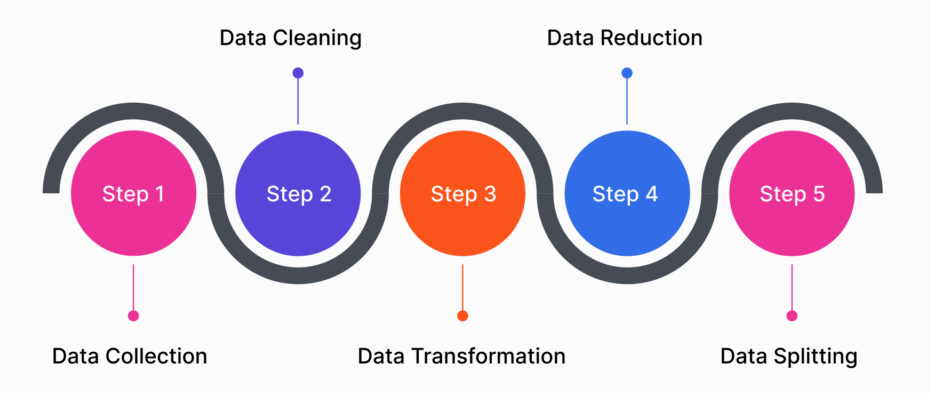
\includegraphics[scale=0.4]{figuras/steps_data_preparing.png}
	\end{center}
	\fonte{\cite{pecan_data_prep_2023}}
\end{figure}

\section{Coleta de dados}

Considerando a premissa do trabalho, em que a previsão do nível do rio será dada a partir de dados meteorológicos da cidade de Porto Alegre, junto aos dados de monitoramento do nível dos rios que constituem a bacia do Guaíba, duas fontes de dados foram utilizadas. Para os dados meteorológicos, o portal do \glsxtrfull{INMET}\footnote{\url{https://portal.inmet.gov.br/}} foi utilizado, onde foram coletadas as informações de temperatura, umidade relativa do ar, precipitação e velocidade do vento. Já os dados de monitoramento dos rios foram coletados na página do \glsxtrfull{SEMA-RS}\footnote{\url{https://www.saladesituacao.rs.gov.br/dados}} da internet (Sala de situação), onde foram coletados os dados de nível do Lago Guaíba,Caí, Jacuí, Sinos e Gravataí. Os dados meteorológicos foram coletados em formato \glsxtrfull{CSV}, com arquivos separados por ano de monitoramento, com frequência horária. Os dados dos níveis dos rios foram coletados no formato \textit{.xlsx}, com histórico completo de amostragem das informações em frequência de 15 minutos, utilizando a biblioteca \textit{Pandas} do Python.

\section{Pré processamento dos dados}

Antes de seguir para a etapa de limpeza dos dados mostrado na Figura \ref{fig:passos_preparacao}, os dados coletados necessitam de um pré-processamento específico para cada uma das fontes utilizadas. Para os dados meteorológicos, devido às informações estarem separadas por ano de monitoramento, foi necessário concatenar os arquivos de cada ano em um único arquivo, utilizando a função \textit{concat} da biblioteca \textit{Pandas}, removendo o cabeçalho de informações geográficas da estação, ilustrado nas linhas 1 a 8 Figura \ref{fig:base_inmet}. Além disso, foi necessário combinar as duas primeiras colunas e converter o formato de data e hora para o padrão \textit{datetime}, utilizando a função \textit{to\_datetime} da mesma biblioteca. 

\begin{figure}[H]
	\caption{\label{fig:base_inmet}Dados meteorológicos.}
	\begin{center}
		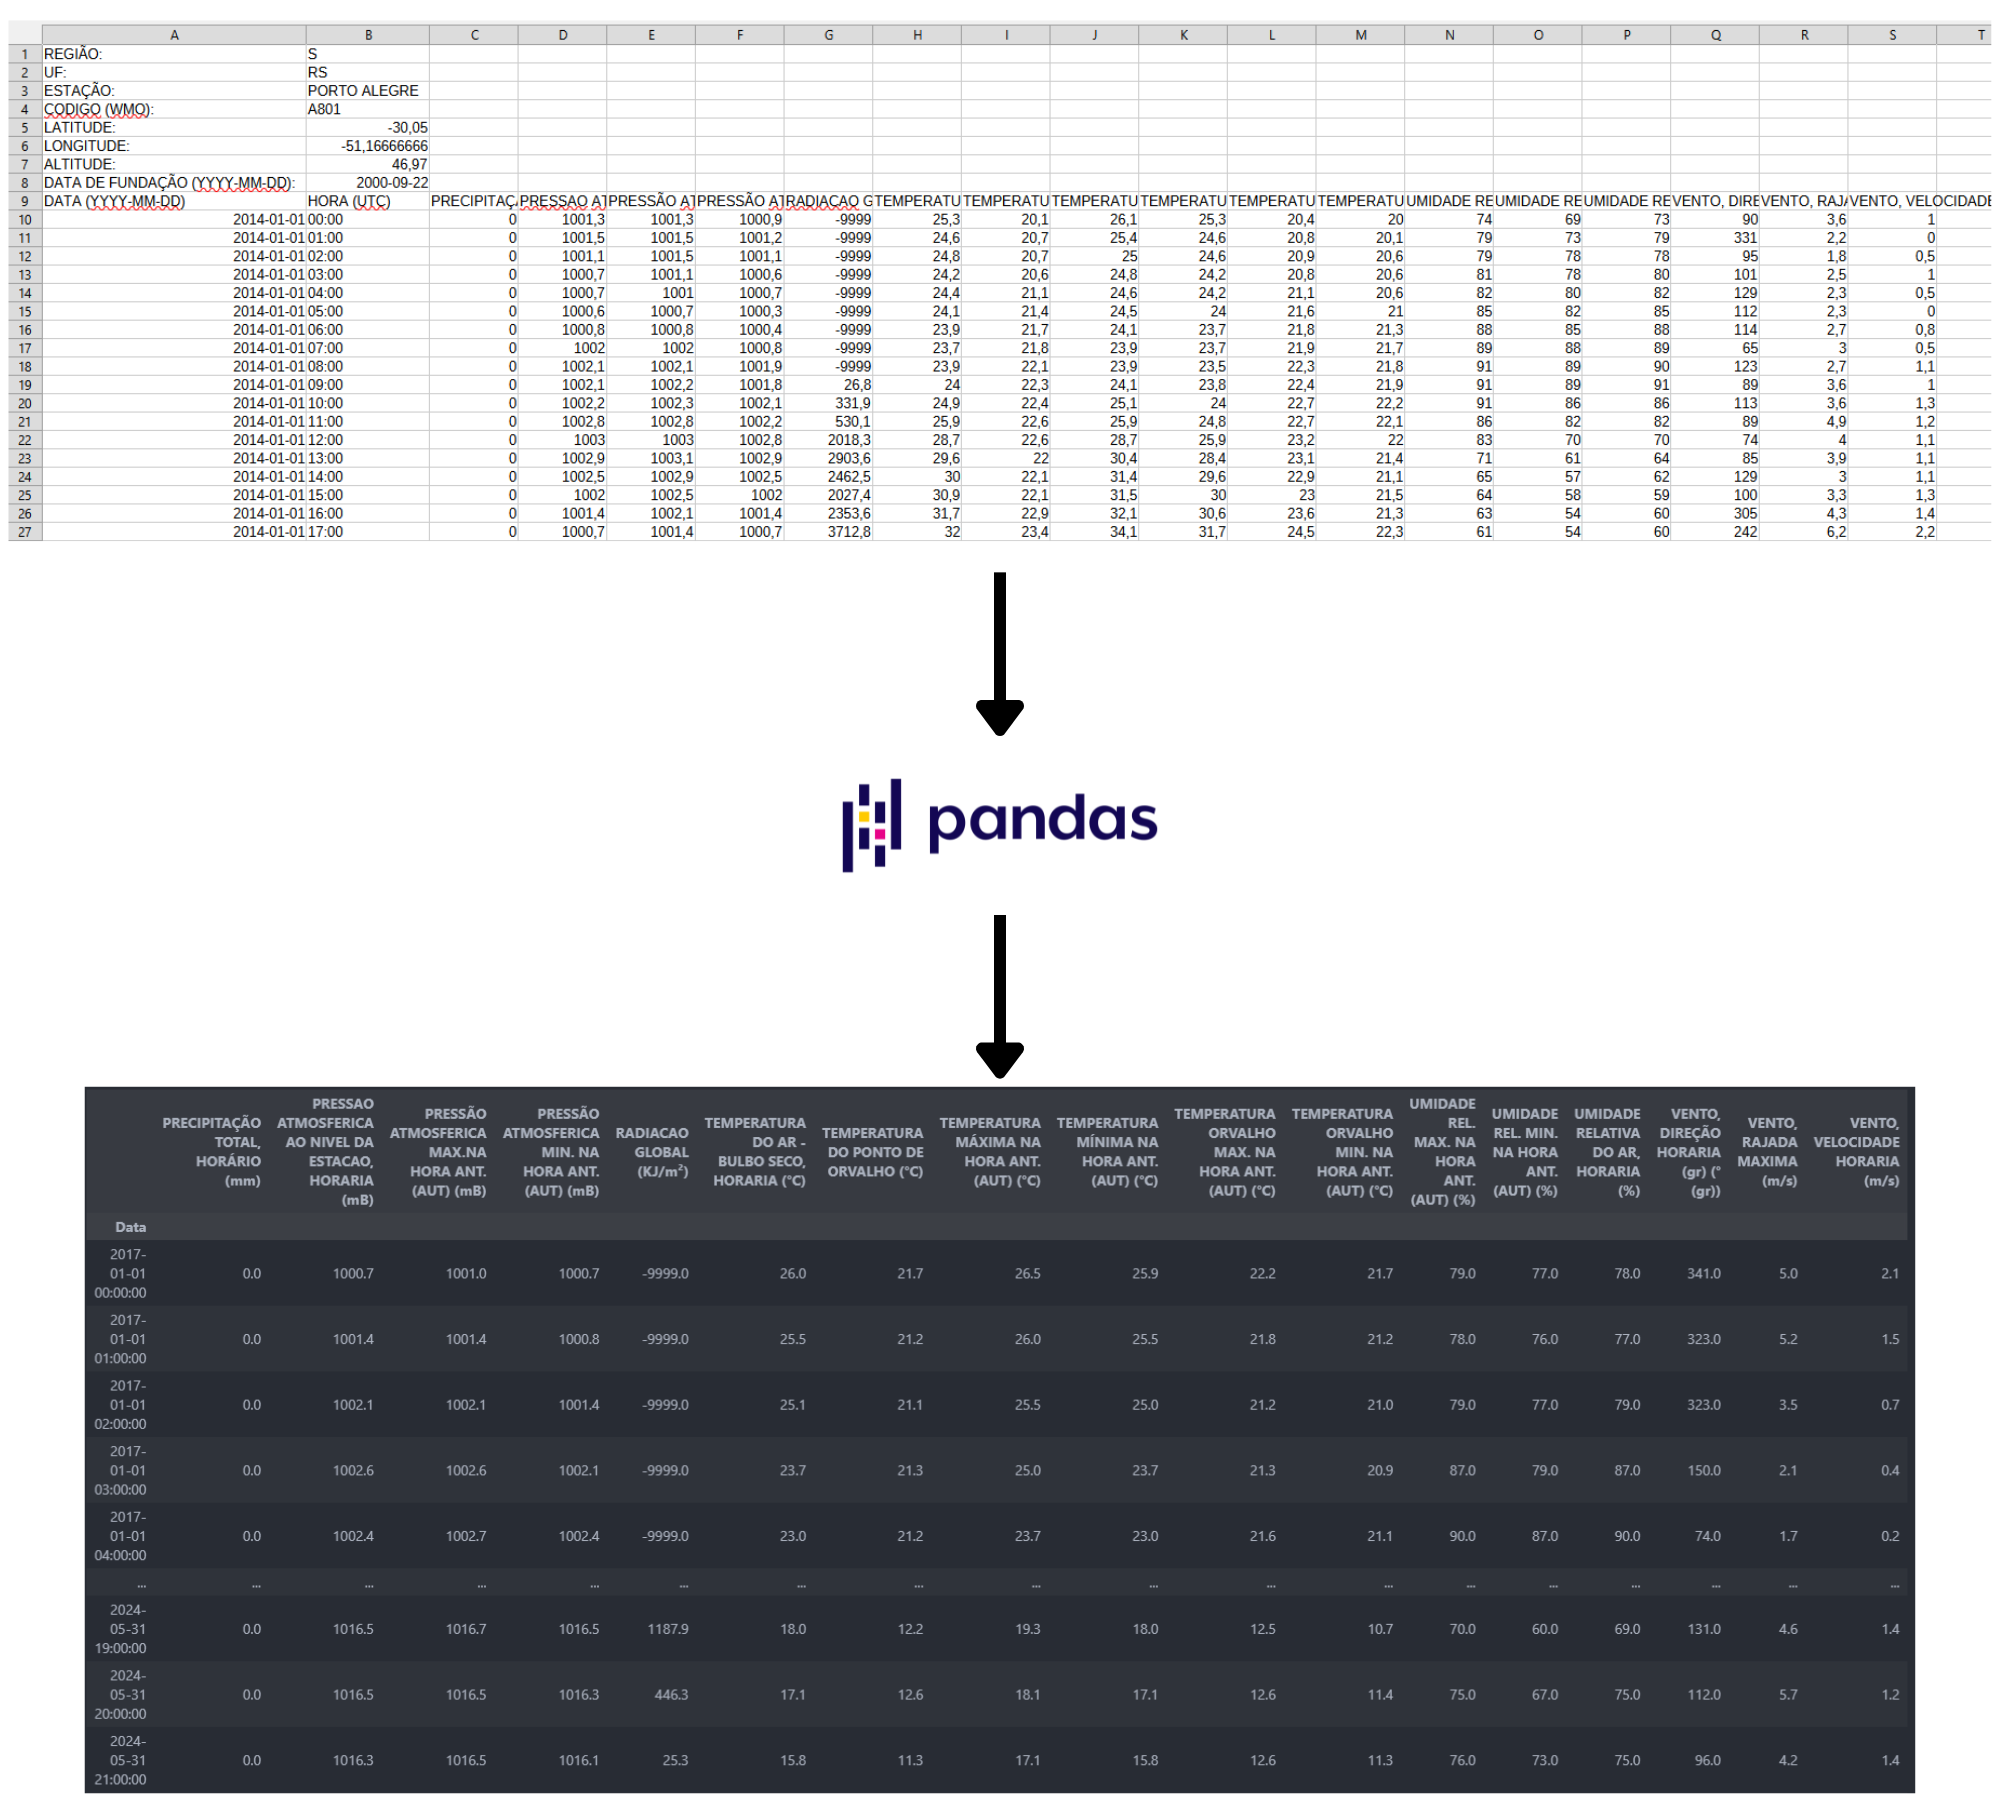
\includegraphics[scale=0.5]{figuras/base_inmet.png}
	\end{center}
	\fonte{Autor.}
\end{figure}

Analisando as colunas e os seus respectivos tipos de dados, tem-se a seguinte tabela:

\begin{table}[H]
	\centering
	\begin{tabular}{|p{10cm}|c|}
	\hline
	\textbf{Coluna} & \textbf{Tipo} \\
	\hline
	Precipitação Total (mm) & float64 \\
	Pressão Atmosférica ao Nível da Estação (mB) & float64 \\
	Pressão Atmosférica Máx. na Hora Anterior (mB) & float64 \\
	Pressão Atmosférica Mín. na Hora Anterior (mB) & float64 \\
	Radiação Global (kJ/m²) & float64 \\
	Temperatura do Ar - Bulbo Seco (°C) & float64 \\
	Temperatura do Ponto de Orvalho (°C) & float64 \\
	Temperatura Máxima na Hora Anterior (°C) & float64 \\
	Temperatura Mínima na Hora Anterior (°C) & float64 \\
	Temperatura Orvalho Máx. na Hora Anterior (°C) & float64 \\
	Temperatura Orvalho Mín. na Hora Anterior (°C) & float64 \\
	Umidade Relativa Máx. na Hora Anterior (\%) & float64 \\
	Umidade Relativa Mín. na Hora Anterior (\%) & float64 \\
	Umidade Relativa do Ar (\%) & float64 \\
	Vento - Direção Horária (° (gr)) & float64 \\
	Vento - Rajada Máxima (m/s) & float64 \\
	Vento - Velocidade Horária (m/s) & float64 \\
	\hline
	\end{tabular}
	\caption{Tabela de tipos de dados da base de informações meteorológicas.}
	\label{tab:colunas_dados_meteorologicos}
\end{table}

Para os dados dos níveis dos rios, também foi necessário remover o cabeçalho com dados geográficos da estação de monitoramento, como mostra a Figura \ref{fig:base_sema}, junto da conversão do formato de data e hora para o padrão \textit{datetime} da primeira coluna.

\begin{figure}[H]
	\caption{\label{fig:base_sema}Dados do nível do rio.}
	\begin{center}
		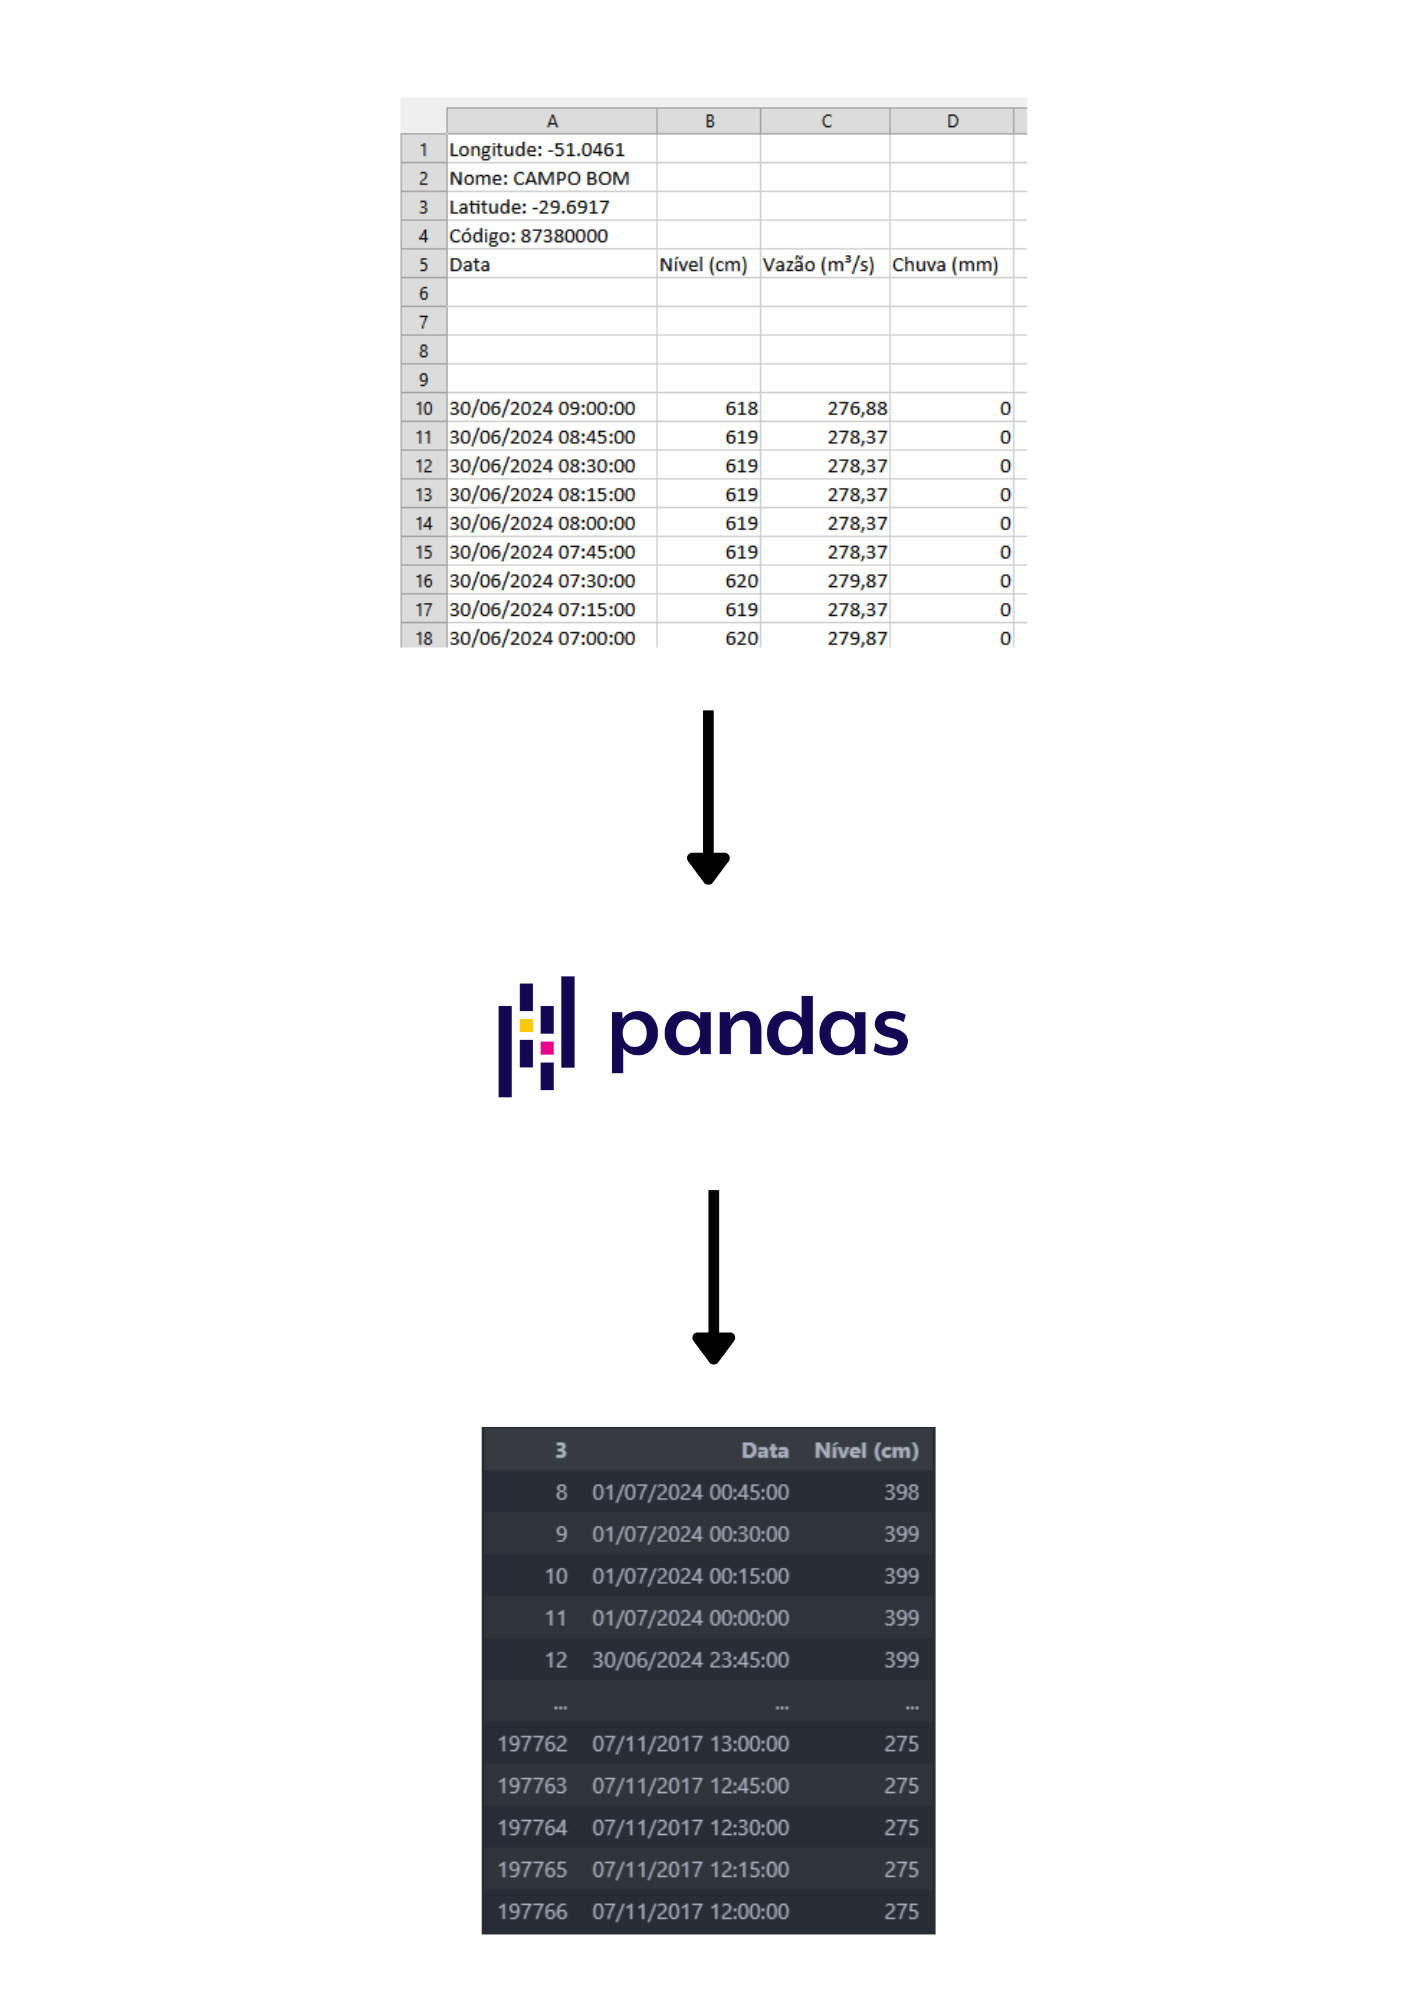
\includegraphics[scale=0.5]{figuras/base_sema.png}
	\end{center}
	\fonte{Autor.}
\end{figure}

\section{Limpeza dos dados}
\label{sec:limpeza_dos_dados}

Após a coleta dos dados, o próximo passo é a limpeza dessas informações, cujo procedimento consiste em remover dados duplicados, corrigir erros de formatação e lidar com valores ausentes. Existem diferentes abordagens para tratar valores inconsistentes no dados coletados. Uma abordagem comum, principalmente em casos onde não há uma linearidade ou tendência clara é o preenchimento com zero \cite{cousineau2010outliers}, como mostra a Figura \ref{fig:passo_dados_limpeza}, ou com a média dos dados na coluna a ser limpa.

\begin{figure}[H]
	\caption{\label{fig:passo_dados_limpeza}Limpeza dos dados coletados.}
	\begin{center}
		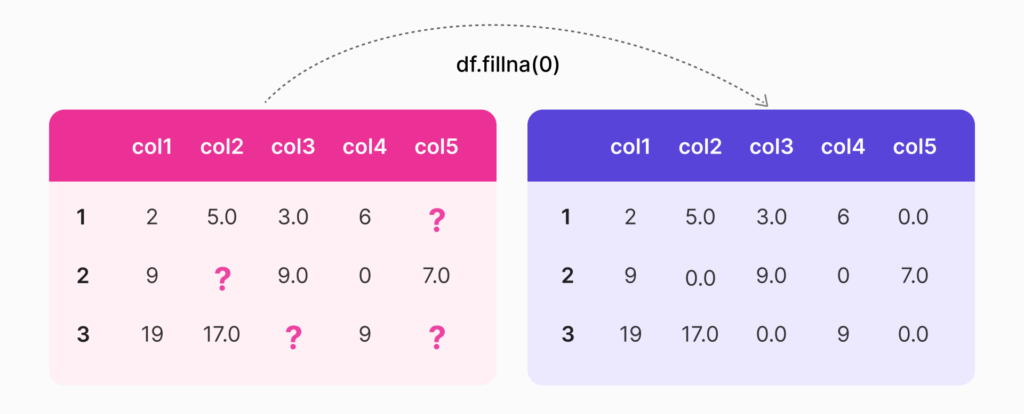
\includegraphics[scale=0.4]{figuras/step_data_cleaning.png}
	\end{center}
	\fonte{\cite{pecan_data_prep_2023}}
\end{figure}

Nessa etapa, na base de dados meteorológicos, optou-se por preencher os dados ausentes, representados por ''-'', e os dados com valor igual a ''-9999'' por zero, já que dados meteorológicos tendem a ser mais voláteis e não apresentam uma tendência clara. Desse modo, a abordagem de aproximação linear é descartada, a fim de não comprometer a análise do modelo de previsão.  

Tomando como exemplo a coluna \textit{TEMPERATURA ORVALHO MAX. NA HORA ANT. (AUT) (°C)}, na Figura \ref{fig:dados_clima_poa_nao_tratados}, observa-se os valores ausentes representados por ''-'' e ''-9999'', evidenciados na Figura pelos pontos distantes do restante dos dados.

\begin{figure}[H]
	\caption{\label{fig:dados_clima_poa_nao_tratados}Gráfico de Temperatura do orvalho Máx. na Hora Anterior (°C) não tratado.}
	\begin{center}
		\includegraphics[scale=0.35]{figuras/TEMPERATURA ORVALHO MAX. NA HORA ANT. (AUT) (°C) SEM TRATAMENTO_edit.png}
	\end{center}
	\fonte{Autor.}
\end{figure}

Após a substituição dos valores ausentes por zero, o gráfico da mesma coluna, mostrado na Figura \ref{fig:dados_clima_poa_tratados}, apresenta uma distribuição mais uniforme, sem os picos de dados ausentes.

\begin{figure}[H]
	\caption{\label{fig:dados_clima_poa_tratados}Gráfico de Temperatura do orvalho Máx. na Hora Anterior (°C) tratado.}
	\begin{center}
		\includegraphics[scale=0.35]{figuras/TEMPERATURA ORVALHO MAX. NA HORA ANT. (AUT) (°C) COM TRATAMENTO.png}
	\end{center}
	\fonte{Autor.}
\end{figure}

Aplicado o tratamento, a coluna \textit{TEMPERATURA ORVALHO MAX. NA HORA ANT. (AUT) (°C)} passa a apresentar uma distribuição mais uniforme, sem os picos de dados ausentes, com valores condizentes com a escala esperada da unidade medida, neste caso, a temperatura em graus Celsius.

Em casos onde os dados apresentam \textit{outliers} (dados que se distanciam significativamente do restante da coluna analisada), foi aplicado o método \glsxtrfull{IQR} para identificar e remover esses valores. A partir da diferença entre o terceiro quartil (Q3) e o primeiro quartil (Q1) de um conjunto de dados, multiplicado por um fator de tolerância, o método determina limites superiores e inferiores para o conjunto de dados analisado, removendo ou substituindo os valores que estão fora dessa faixa, para manter a consistência das informações.

Por exemplo, na coluna \textit{UMIDADE REL. MAX. NA HORA ANT. (AUT) (\%)}, as Figuras \ref{fig:dados_outlier_sem_tratamento} e \ref{fig:dados_outlier_com_tratamento} mostram a diferença entre os dados após a aplicação do método \gls{IQR}, com um fator de tolerância de 1.2 entre os interquartis Q1 e Q3. Para esta coluna, o cálculo do IQR resultou em um intervalo de -11,8\% a 35,8\%, limitando os \textit{outliers} superiores vistos no gráfico para o valor máximo calculado. 

\begin{figure}[H]
	\caption{\label{fig:dados_outlier_sem_tratamento}Gráfico de Umidade Relativa Máxima  na Hora Anterior (\%) sem tratamento.}
	\begin{center}
		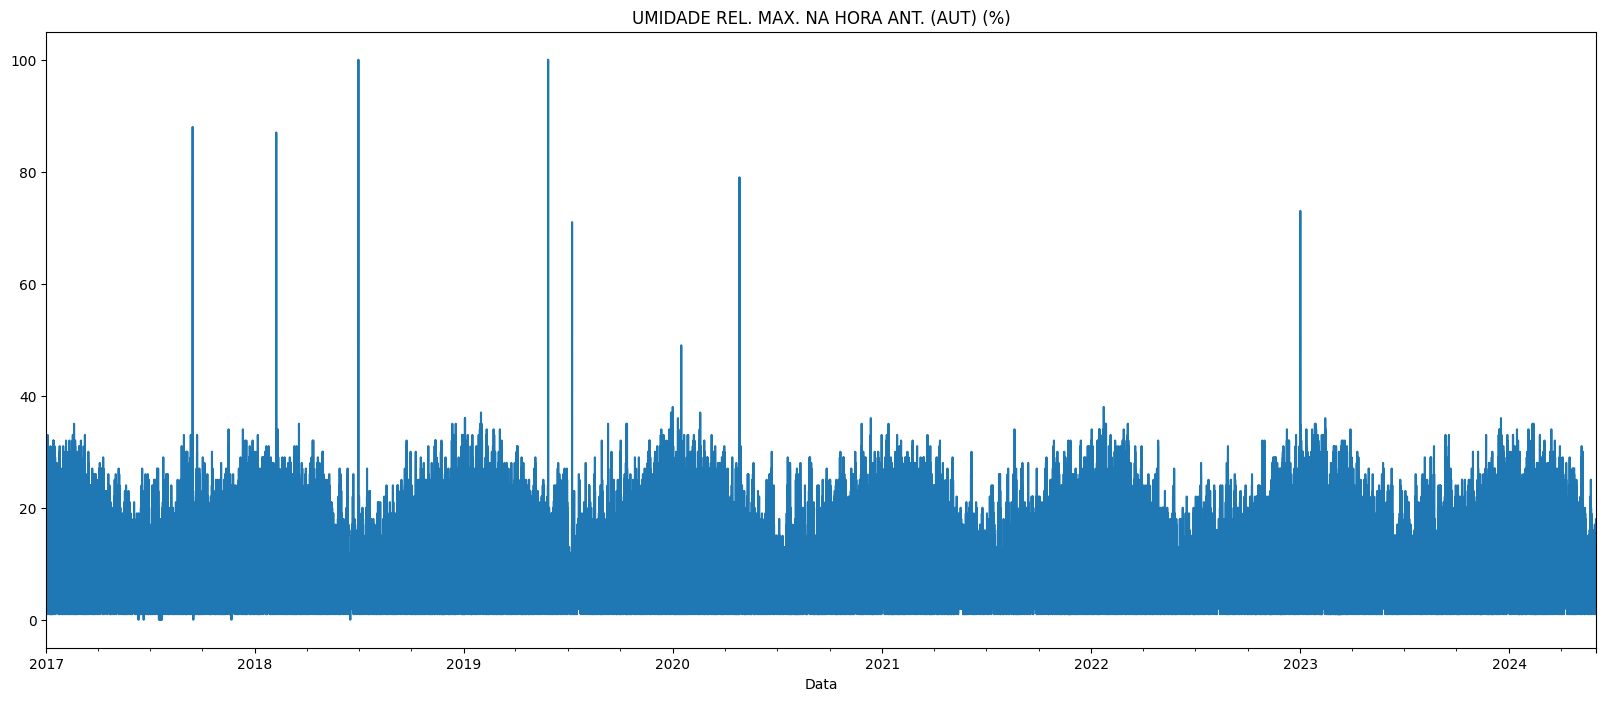
\includegraphics[scale=0.35]{figuras/UMIDADE REL. MAX. NA HORA ANT. (AUT) SEM TRATAMENTO.png}
	\end{center}
	\fonte{Autor.}
\end{figure}

\begin{figure}[H]
	\caption{\label{fig:dados_outlier_com_tratamento}Gráfico de Umidade Relativa Máxima  na Hora Anterior (\%) com tratamento.}
	\begin{center}
		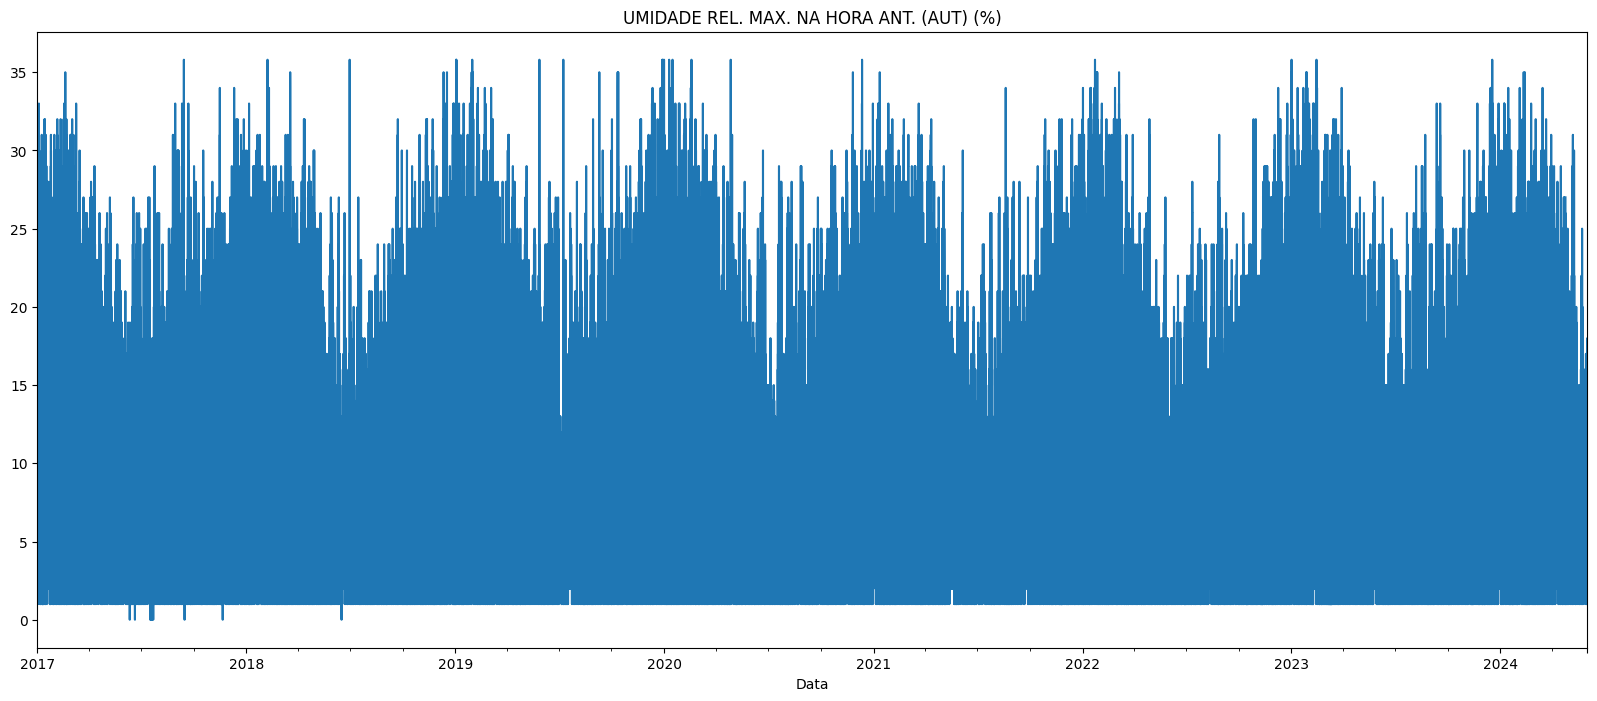
\includegraphics[scale=0.35]{figuras/UMIDADE REL. MAX. NA HORA ANT. (AUT) COM TRATAMENTO.png}
	\end{center}
	\fonte{Autor.}
\end{figure}

Na base de dados dos níveis dos rios, embora a dinâmica que representa os respectivos comportamentos não seja linear, o uso do conceito de aproximação linear permite preencher os dados ausentes por meio da interpolação entre os valores que cercam as células sem informação em determinado período. Essa abordagem é válida, uma vez que a variação do nível do rio entre dois pontos de amostragem próximos tende a ser linear, já que o nível do rio não apresenta oscilações bruscas em curtos períodos de tempo.

Para realizar a interpolação, utilizou-se a função \textit{interpolate} com o argumento \textit{method = linear} da biblioteca \textit{Pandas}, que preenche os valores ausentes com base nos dados adjacentes.

Para realizar a interpolação dos valores ausentes na base de dados dos níveis dos rios, utilizou-se a função \textit{interpolate} da biblioteca Pandas com o argumento \textit{method = 'linear'}. Esse método preenche os valores ausentes calculando uma interpolação linear entre os dois dados adjacentes mais próximos, ou seja, o valor ausente é estimado como uma média ponderada dos valores imediatamente anteriores e posteriores no conjunto de dados, considerando a distância temporal entre eles. Especificamente, a interpolação linear utiliza apenas os dois pontos adjacentes (um antes e um depois do valor ausente) para determinar o valor interpolado, assumindo uma variação linear entre esses pontos.

Ainda, observou-se nas bases dos níveis dos rios a ocorrência de valores ausentes no início ou no final do período de amostragem, inviabilizando a interpolação. Para esses casos, o preenchimento foi feito a partir da repetição do primeiro ou do último valor disponível, respectivamente. É importante ressaltar que tal limpeza só pode ser feita se o preenchimento ocorra em um intervalo de tempo curto, visando não afetar a análise feita pelo modelo de previsão.

\section{Redução dos dados}

A etapa de redução dos dados visa eliminar informações redundantes ou irrelevantes, mantendo apenas os dados que contribuem para a análise e treinamento do modelo de previsão. Considerando que serão utilizados dados de monitoramento do nível de 4 rios para a previsão do nível do Lago Guaíba, os dados meteorológicos coletados precisam ser filtrados de modo a garantir tanto que as informações sejam relevantes para a previsão, quanto que os dados de monitoramento dos rios estejam alinhados com os dados meteorológicos, evitando assim a inclusão de dados desnecessários no treinamento. 

Voltando para a Tabela \ref{tab:colunas_dados_meteorologicos}, nota-se a presença de 17 colunas, das quais:

\begin{itemize}
	\item 6 colunas referem-se a dados de temperatura;
	\item 3 colunas referem-se a dados de pressão atmosférica;
	\item 3 colunas referem-se a dados do comportamento do vento;
	\item 3 colunas referem-se a dados de umidade relativa do ar;
	\item 1 coluna refere-se a dados de radiação solar.
	\item 1 coluna refere-se a dados de precipitação.
\end{itemize}

Desse modo, para o primeiro passo de redução da base, foram mantidas apenas uma coluna de cada tipo de medição meteorológica, filtrando 6 colunas no total, conforme a Tabela \ref{tab:colunas_dados_meteorologicos_reduzidas}. 

\begin{table}[H]
	\centering
	\begin{tabular}{|p{10cm}|c|}
	\hline
	\textbf{Coluna} & \textbf{Unidade de medida} \\
	\hline
	Temperatura do Ar - Bulbo seco & (°C) \\
	Pressão Atmosférica ao Nível da Estação & (mB) \\
	Vento - Velocidade Horária & (m/s) \\
	Umidade Relativa do Ar & (\%) \\
	Radiação Global & (kJ/m²) \\
	Precipitação Total & (mm) \\
	\hline
	\end{tabular}
	\caption{Tabela de dados meteorológicos reduzidos - 1ª Filtragem}
	\label{tab:colunas_dados_meteorologicos_reduzidas}
\end{table}

Para a escolha das colunas a serem mantidas, foram levados em consideração os seguintes critérios:
\begin{itemize}
	\item As colunas \textit{Temperatura do Ar - Bulbo seco}, \textit{Pressão Atmosférica ao Nível da Estação} e \textit{Umidade Relativa do Ar} foram escolhidas por serem medidas diretas dos respectivos fenômenos atmosféricos, enquanto as demais colunas referem-se a medidas derivadas ou não diretamente observáveis, que não são tão relevantes para a previsão do nível do rio. Além disso, observou-se que para essas unidades de medida derivadas, o comportamento dos dados eram semelhantes, descartando a necessidade de manter mais de uma coluna para cada tipo de medição, como mostra a Figura \ref{fig:comparacao_temp} em relação às medidas de temperatura.
	\begin{figure}[H]
	\caption{\label{fig:comparacao_temp}Comparativo de gráficos de temperatura em diferentes tipos de medição}
	\begin{center}
		\begin{subfigure}{0.35\textwidth}
			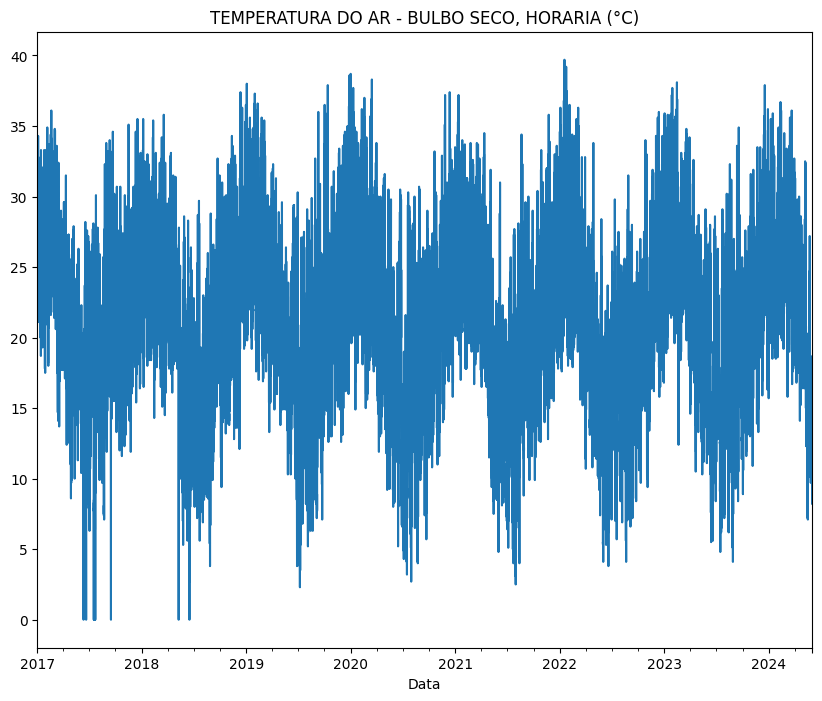
\includegraphics[width=\linewidth]{figuras/comparacao_temp_1.png}
		\end{subfigure}
		\begin{subfigure}{0.35\textwidth}
			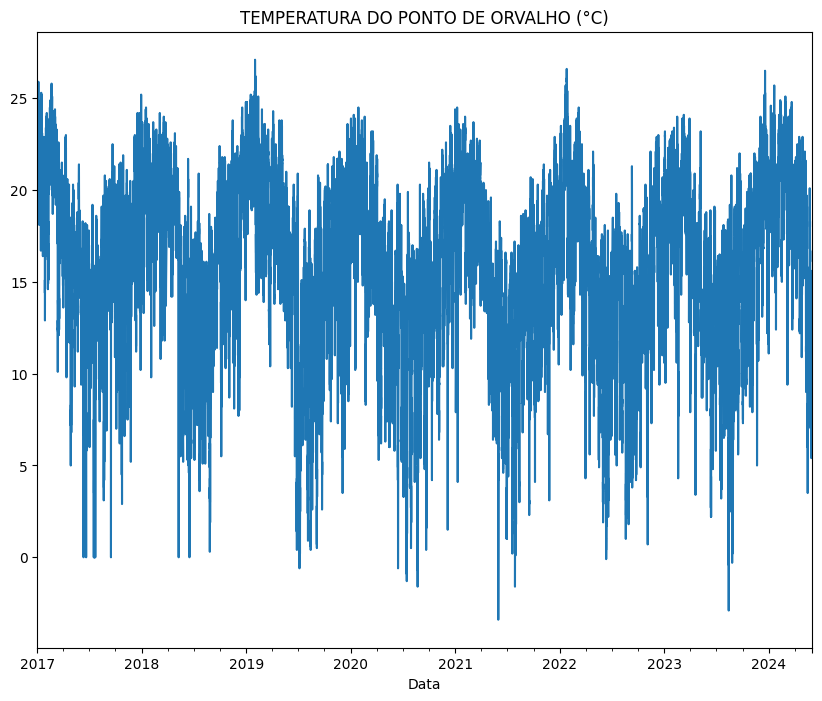
\includegraphics[width=\linewidth]{figuras/comparacao_temp_2.png}
		\end{subfigure}
		
		\begin{subfigure}{0.35\textwidth}
			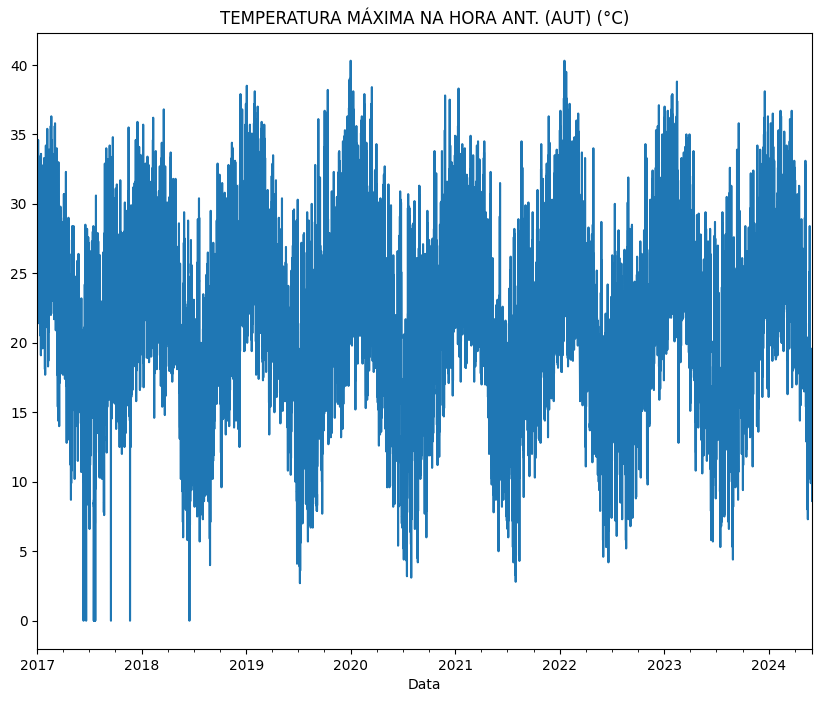
\includegraphics[width=\linewidth]{figuras/comparacao_temp_3.png}
		\end{subfigure}
		\begin{subfigure}{0.35\textwidth}
			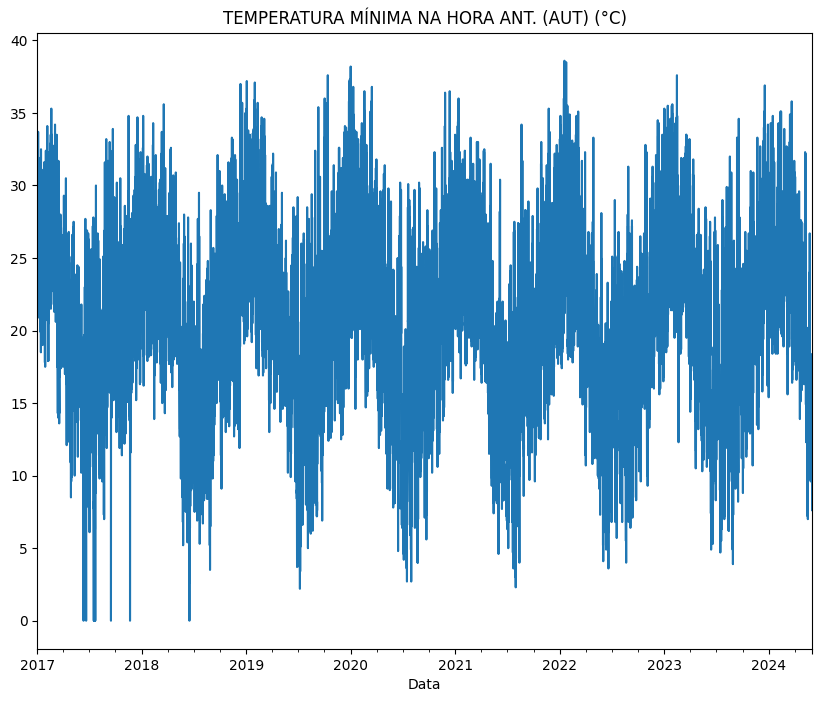
\includegraphics[width=\linewidth]{figuras/comparacao_temp_4.png}
		\end{subfigure}
		
		\begin{subfigure}{0.35\textwidth}
			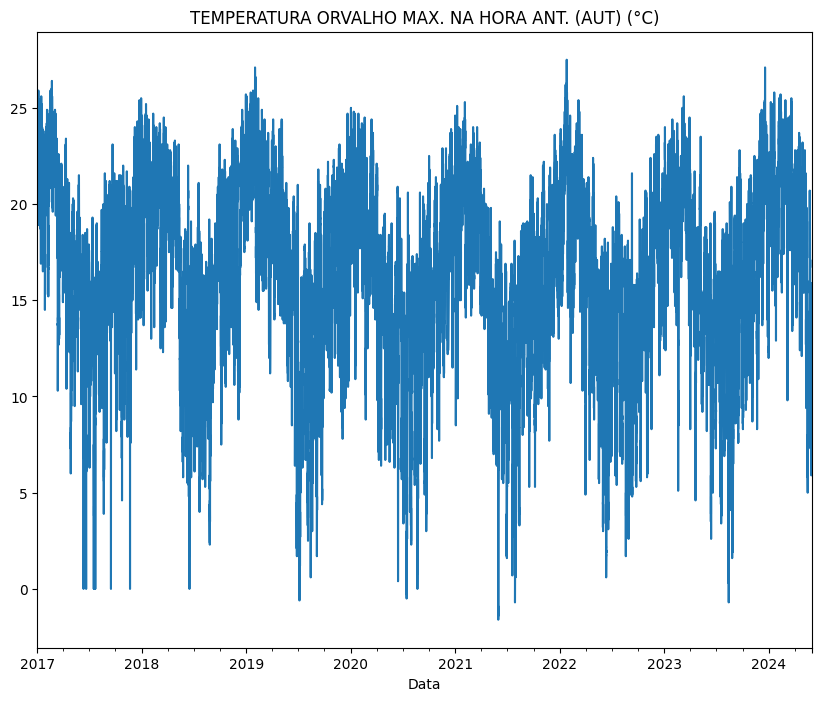
\includegraphics[width=\linewidth]{figuras/comparacao_temp_5.png}
		\end{subfigure}
		\begin{subfigure}{0.35\textwidth}
			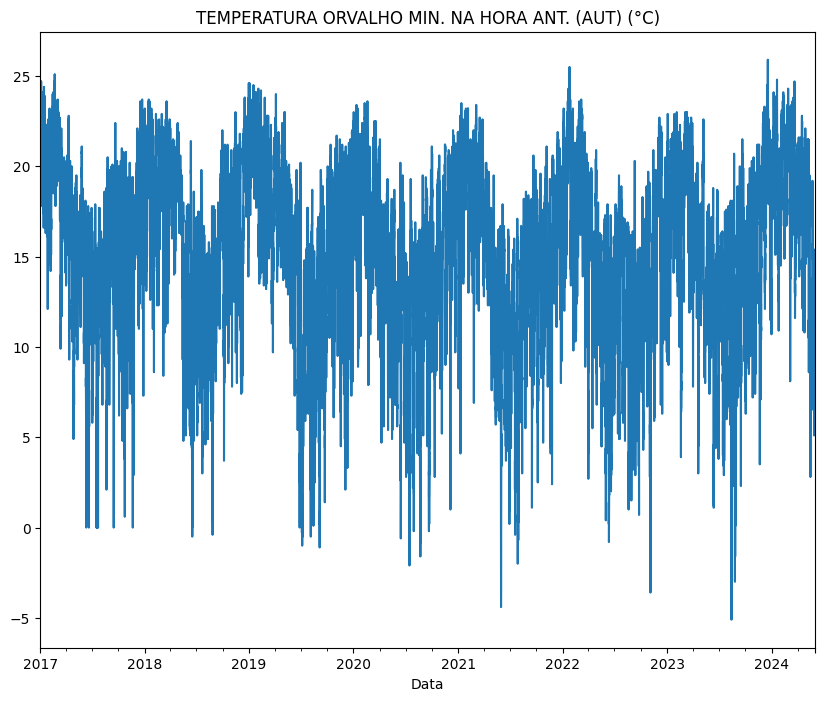
\includegraphics[width=\linewidth]{figuras/comparacao_temp_6.png}
		\end{subfigure}
	\end{center}
	\fonte{Autor.}
	\end{figure}
	\item A coluna \textit{Precipitação Total} foi mantida por ser um dos principais fatores que influenciam o nível do rio.
	\item As colunas \textit{Radiação Global} e \textit{Umidade Relativa do Ar} foram mantidas por serem fatores importantes para a evaporação da água, que também influenciam, mesmo que de forma indireta, no nível do rio.
\end{itemize}

Após essa redução inicial, os gráficos e seus dados de cada coluna foram analisados, a fim de verificar se as informações eram consistentes e poderiam contribuir para o treinamento do modelo. Nas Figuras \ref{fig:temperatura_do_ar_bulbo_seco}, \ref{fig:pressao_atmosferica_ao_nivel_da_estacao}, \ref{fig:vento_velocidade_horaria}, \ref{fig:umidade_relativa_do_ar}, \ref{fig:radiacao_global} e \ref{fig:precipitacao_total}, são apresentados os gráficos de cada uma das colunas mantidas.

\begin{figure}[H]
	\caption{\label{fig:temperatura_do_ar_bulbo_seco}Gráfico de Temperatura do Ar - Bulbo Seco}
	\begin{center}
		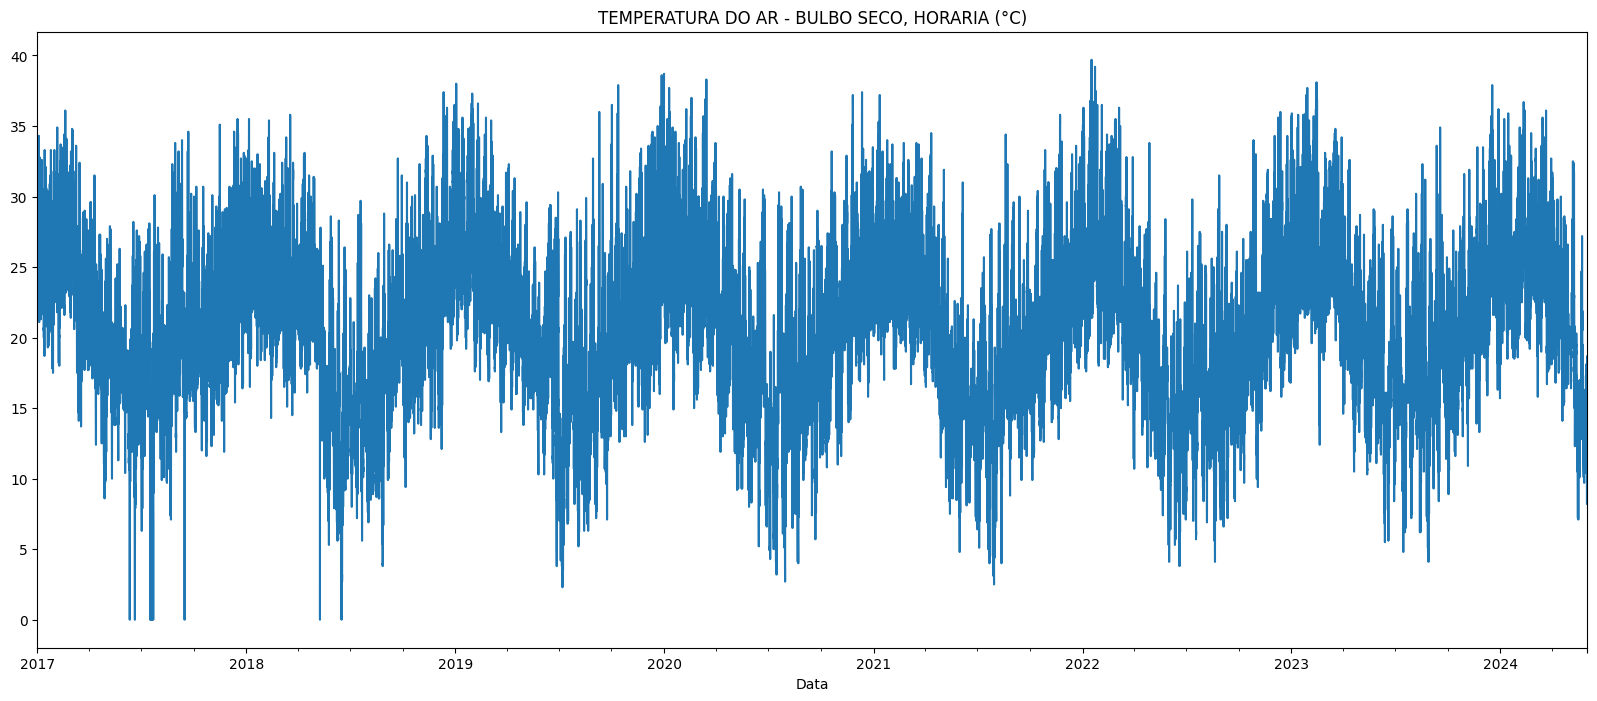
\includegraphics[scale=0.35]{figuras/temperatura_do_ar_bulbo_seco.png}
	\end{center}
	\fonte{Autor.}
\end{figure}

\begin{figure}[H]
	\caption{\label{fig:pressao_atmosferica_ao_nivel_da_estacao}Gráfico de Pressão Atmosférica ao Nível da Estação.}
	\begin{center}
		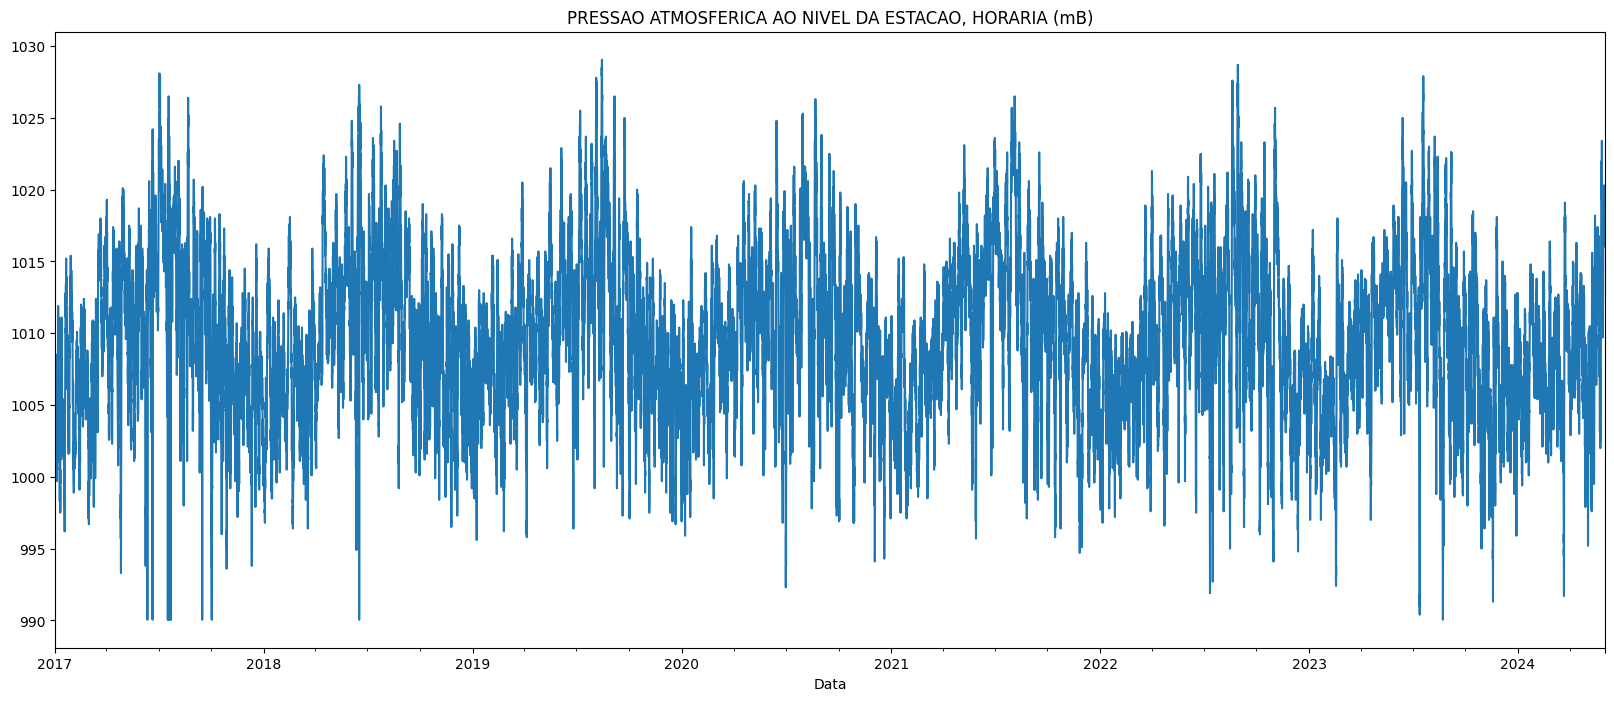
\includegraphics[scale=0.35]{figuras/pressao_atmosferica_ao_nivel_da_estacao.png}
	\end{center}
	\fonte{Autor.}
\end{figure}

\begin{figure}[H]
	\caption{\label{fig:vento_velocidade_horaria}Gráfico de Vento - Velocidade Horária.}
	\begin{center}
		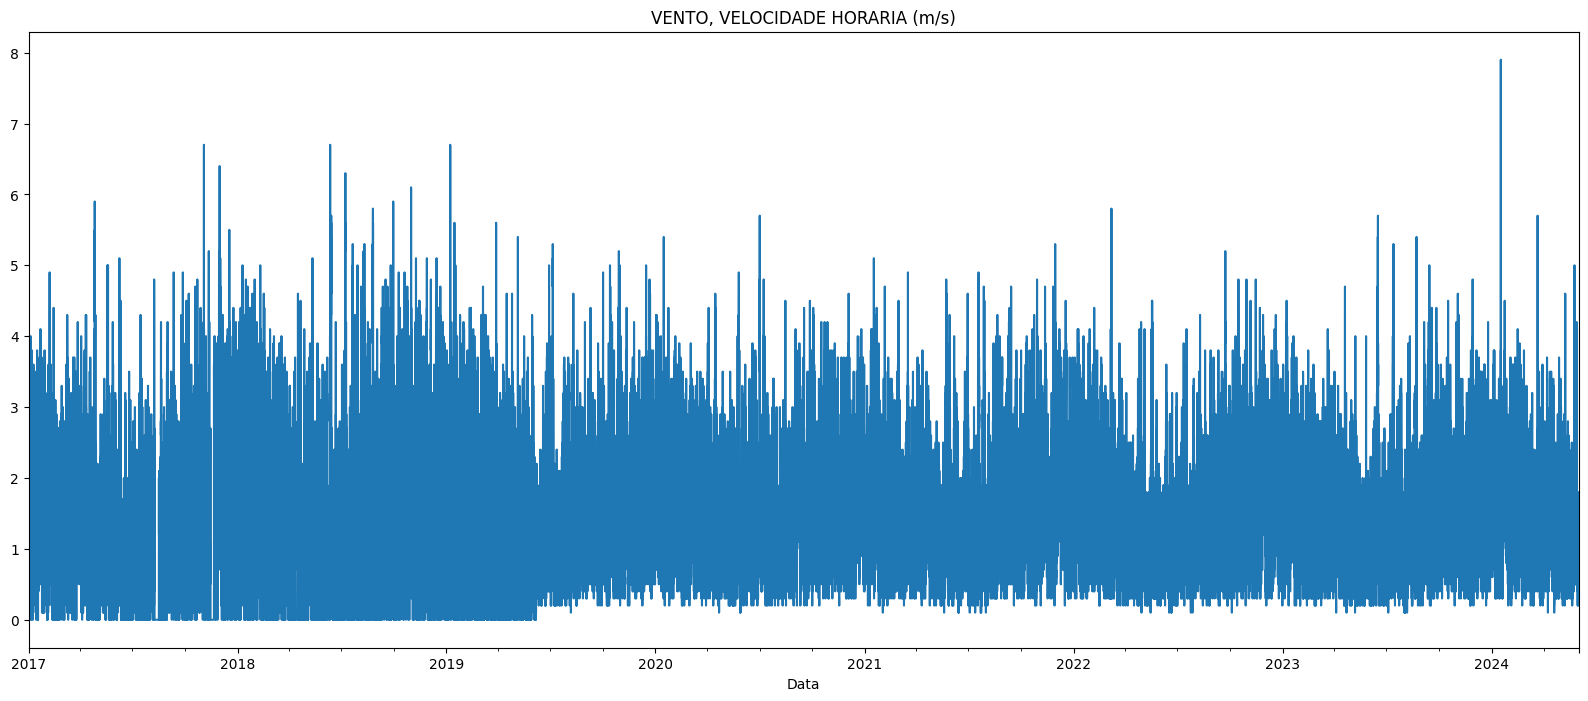
\includegraphics[scale=0.35]{figuras/vento_velocidade_horaria.png}
	\end{center}
	\fonte{Autor.}
\end{figure}

\begin{figure}[H]
	\caption{\label{fig:umidade_relativa_do_ar}Gráfico de Umidade Relativa do Ar}
	\begin{center}
		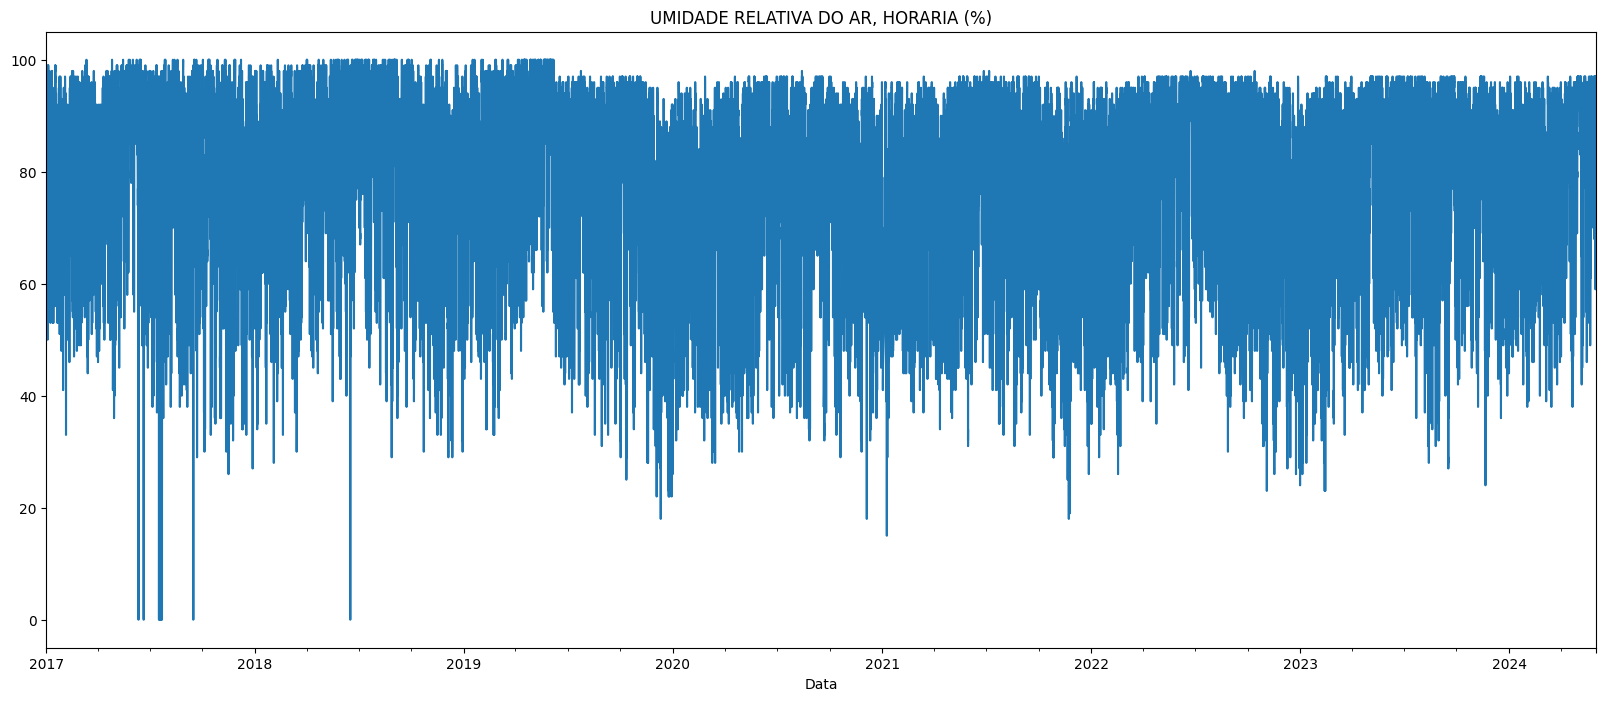
\includegraphics[scale=0.35]{figuras/umidade_relativa_do_ar.png}
	\end{center}
	\fonte{Autor.}
\end{figure}

\begin{figure}[H]
	\caption{\label{fig:radiacao_global}Gráfico de Radiação Global}
	\begin{center}
		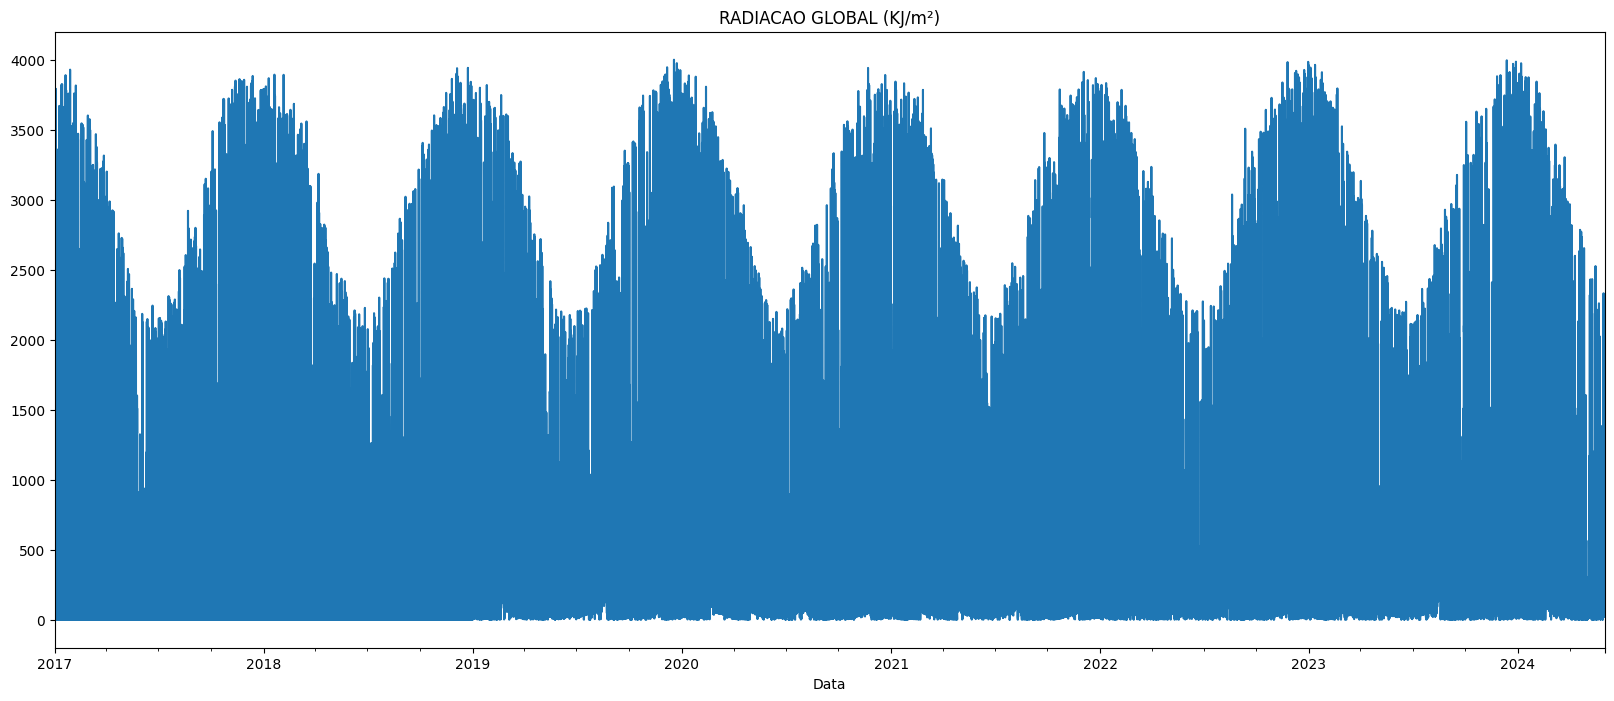
\includegraphics[scale=0.35]{figuras/radiacao_global.png}
	\end{center}
	\fonte{Autor.}
\end{figure}

\begin{figure}[H]
	\caption{\label{fig:precipitacao_total}Gráfico de Precipitação Total}
	\begin{center}
		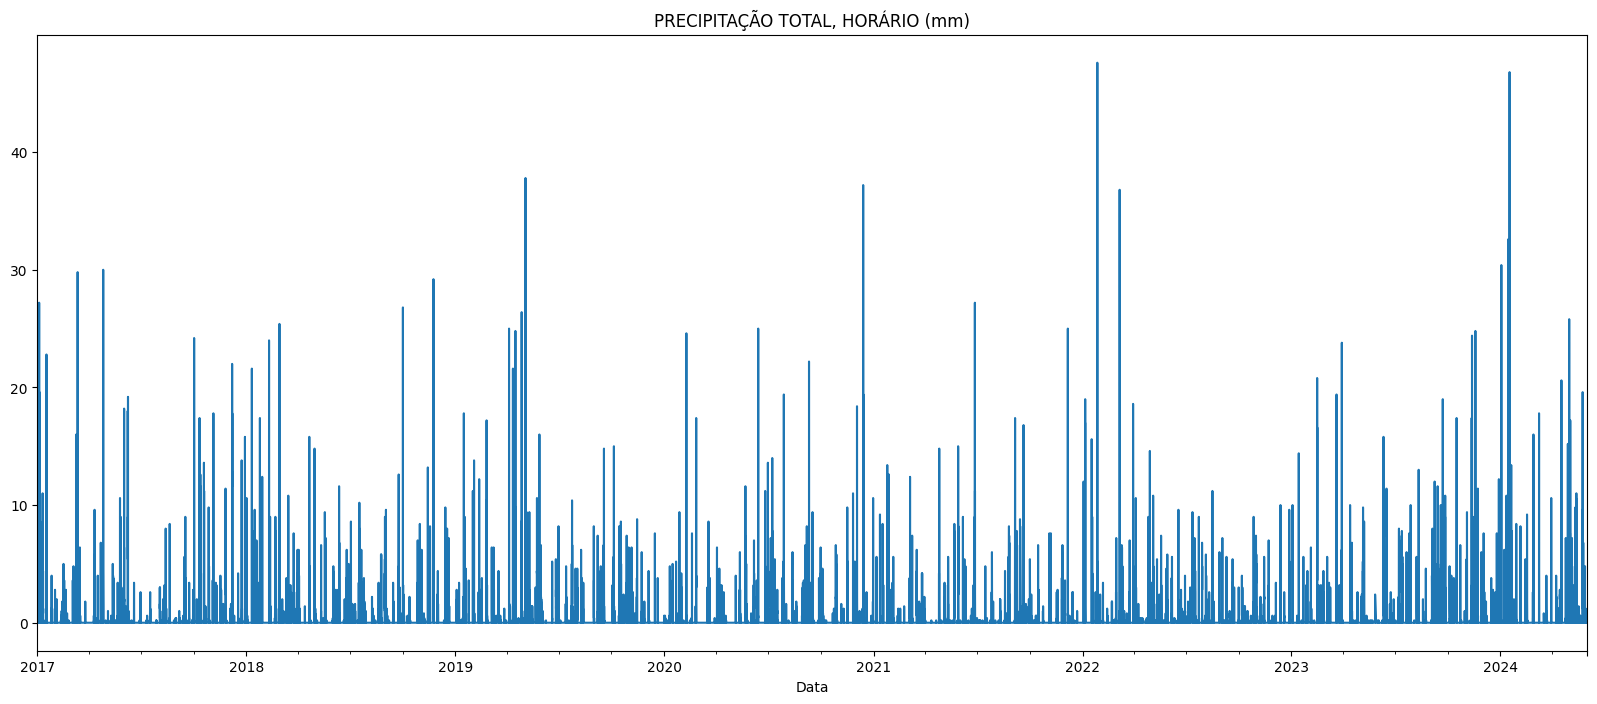
\includegraphics[scale=0.35]{figuras/precipitacao_total_horario.png}
	\end{center}
	\fonte{Autor.}
\end{figure}

As Figuras \ref{fig:temperatura_do_ar_bulbo_seco}, \ref{fig:pressao_atmosferica_ao_nivel_da_estacao} e \ref{fig:radiacao_global} ilustram um padrão sazonal nos dados, com aumentos e diminuições periódicas dos valores ao longo do ano, indicando uma correlação entre as variáveis meteorológicas e as estações do ano. Desse modo, torna-se justificável a manutenção dessas colunas, uma vez que o modelo de previsão pode se beneficiar dessa sazonalidade para melhorar a acurácia das previsões, considerando que o nível do rio também apresenta a mesma dinâmica, ilustrado nas Figuras \ref{fig:comparacao_temp_nivel_rio}, \ref{fig:comparacao_pressao_nivel_rio} e \ref{fig:comparacao_radiacao_nivel_rio}.

\begin{figure}[H]
	\caption{\label{fig:comparacao_temp_nivel_rio}Gráfico comparativo de temperatura e nível quanto a sazonalidade}
	\begin{center}
		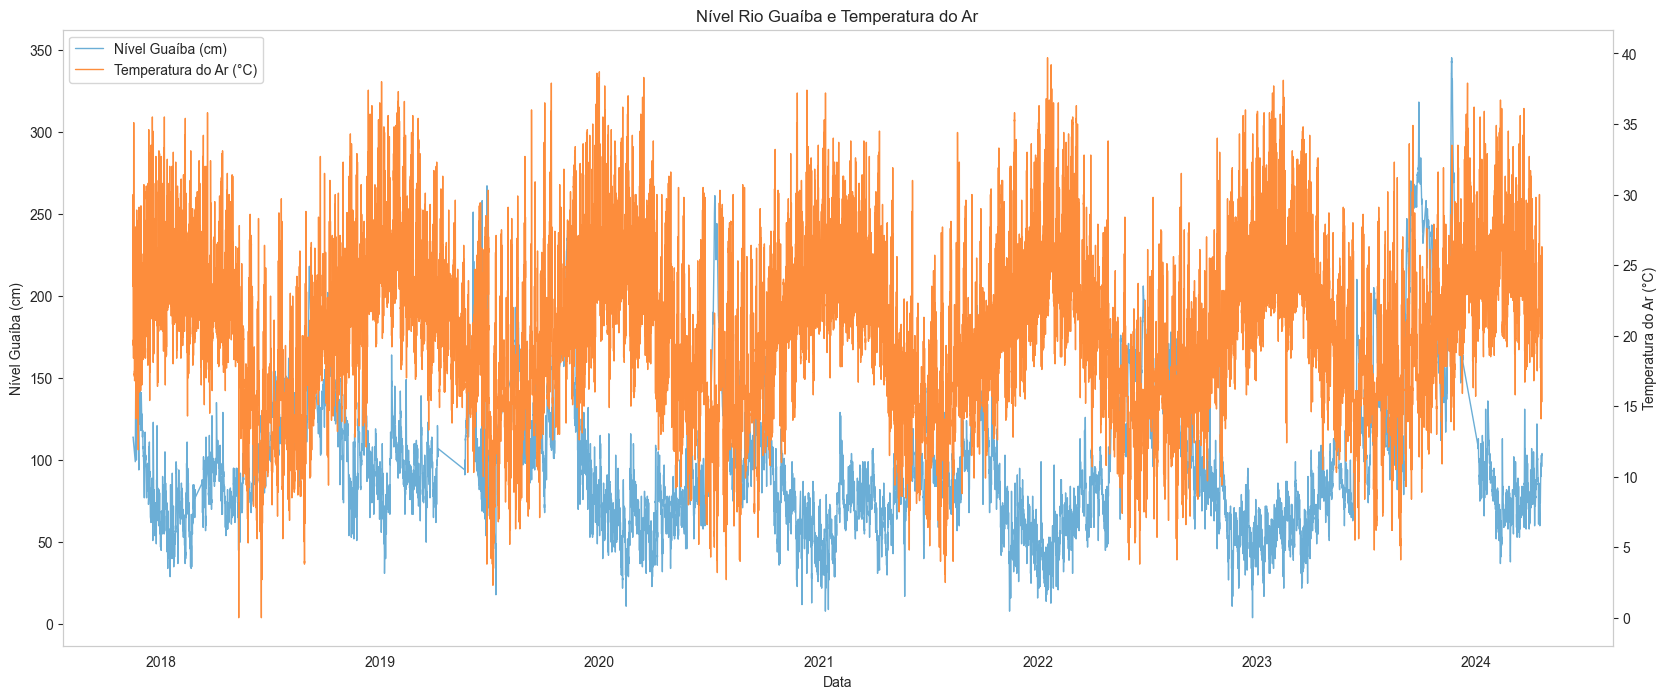
\includegraphics[scale=0.35]{figuras/comparacao_temp_nivel_rio.png}
	\end{center}
	\fonte{Autor.}
\end{figure}

\begin{figure}[H]
	\caption{\label{fig:comparacao_pressao_nivel_rio}Gráfico comparativo de pressão atmosférica e nível quanto a sazonalidade}
	\begin{center}
		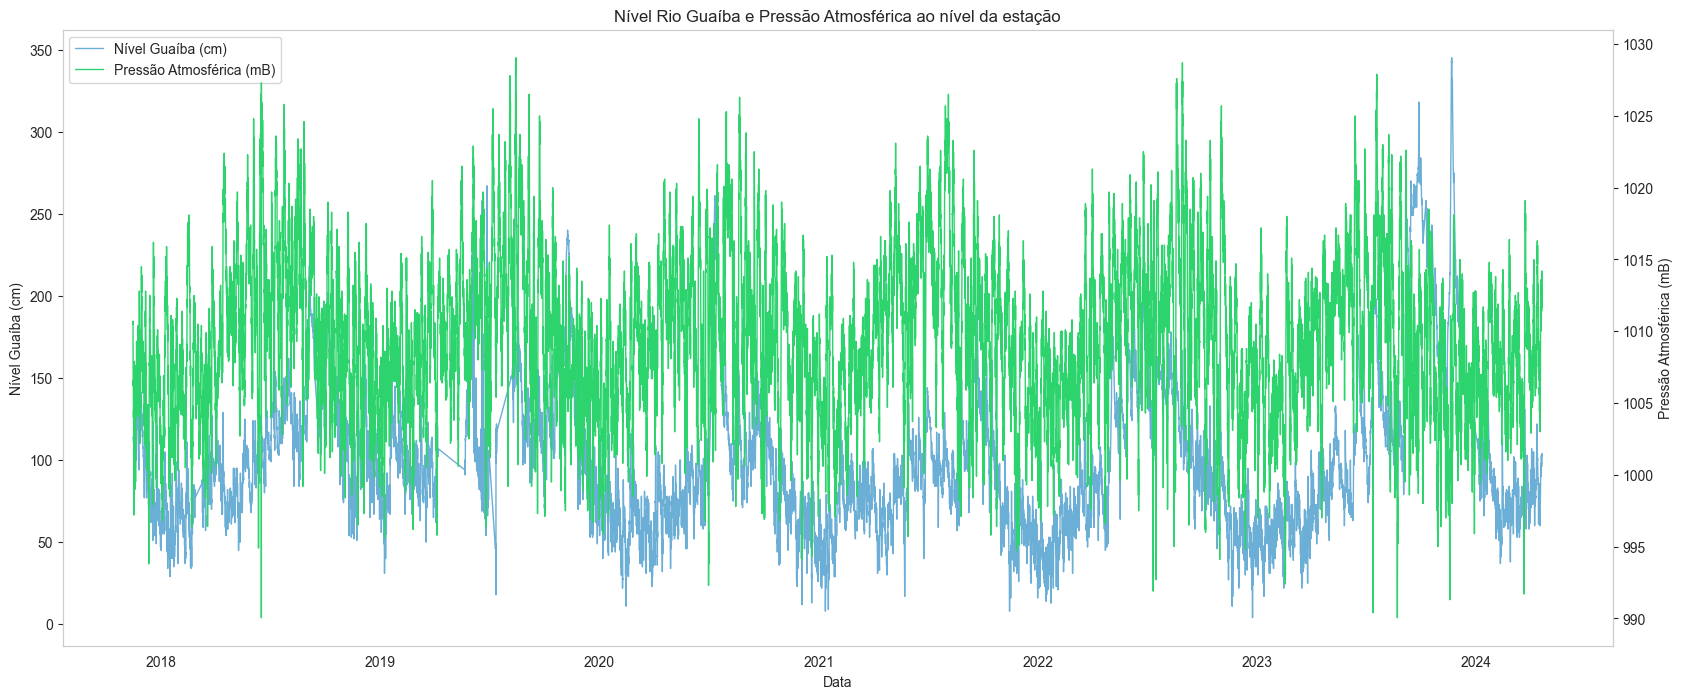
\includegraphics[scale=0.35]{figuras/comparacao_pressao_nivel_rio.png}
	\end{center}
	\fonte{Autor.}
\end{figure}

\begin{figure}[H]
	\caption{\label{fig:comparacao_radiacao_nivel_rio}Gráfico comparativo de radiação global e nível quanto a sazonalidade}
	\begin{center}
		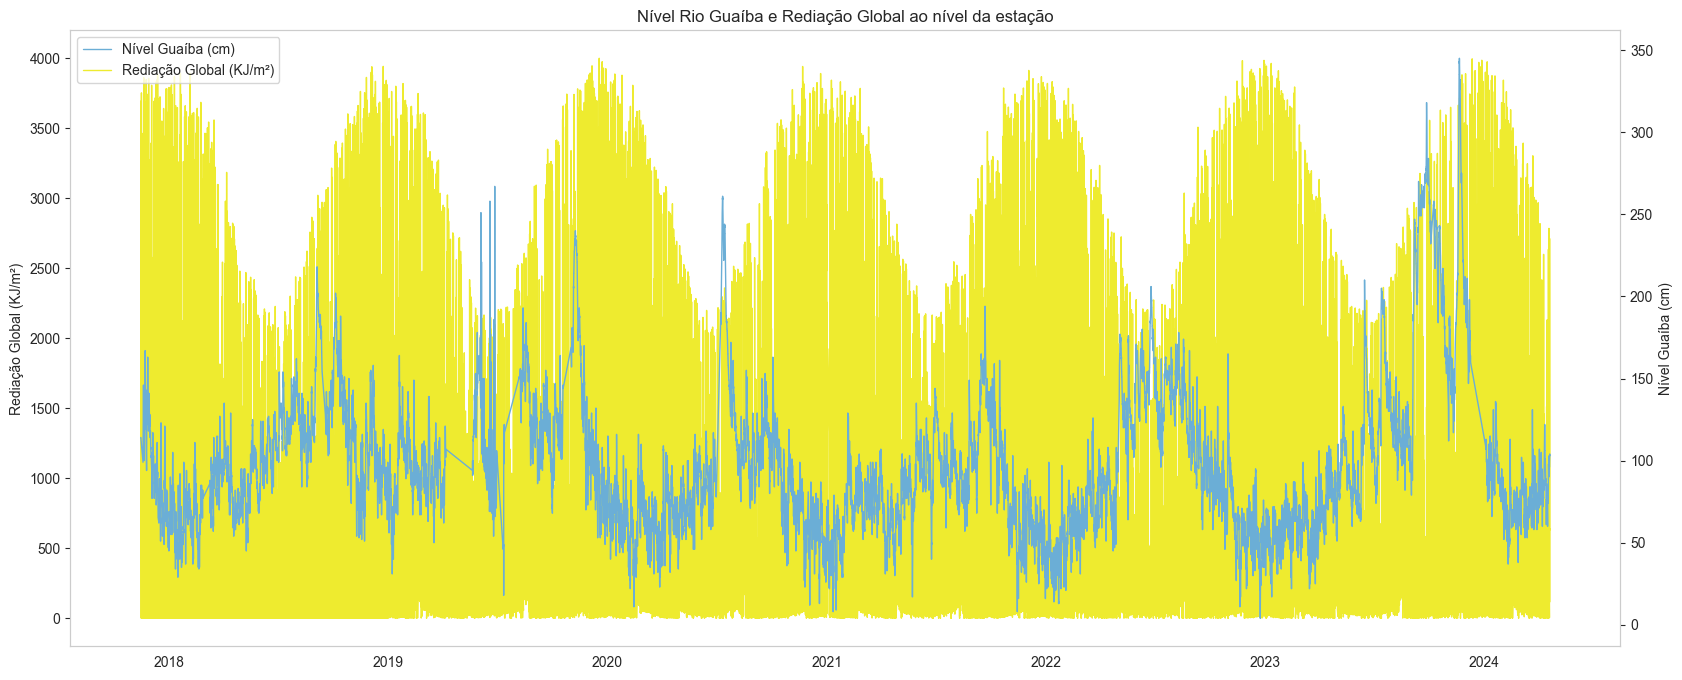
\includegraphics[scale=0.35]{figuras/comparacao_radiacao_nivel_rio.png}
	\end{center}
	\fonte{Autor.}
\end{figure}

Em relação às colunas \textit{Vento - Velocidade Horária}, \textit{Umidade Relativa do Ar} e \textit{Precipitação Total}, embora estas não apresentem um padrão sazonal tão evidente quanto as plotadas acima, estas medidas estão diretamente ligadas aos fenômenos de previsão do tempo, noticiadas em jornais e revistas, e portanto, possuem influência direta no nível dos rios ondes estes dados são monitorados. Sendo assim, as colunas também foram consideradas para o treinamento do modelo.

Definidas as colunas a serem mantidas, o próximo passo consistiu em alinhar os dados meteorológicos com os dados de monitoramento dos rios, garantindo que as informações estivessem na mesma frequência de amostragem. Para isso, foram utilizados os dados de monitoramento do nível do Lago Guaíba, que possuem a maior frequência de amostragem entre os rios analisados, com intervalo de 15 minutos, enquanto os dados meteorológicos possuem frequência de 1 hora (60 minutos). Assim, a frequência de amostragem das informações do nível dos rios foi reduzida para 1 hora, aplicando um filtro simples que mantém apenas as linhas cujo \textit{timestamp} tem minuto igual a 0.

Por fim, alinhados os dados meteorológicos com os dados de monitoramento dos rios, o \textit{dataframe} resultante passou por um nivelamento superior e inferior quanto a data inicial e final, visando manter um período de amostragem em que todas as colunas possuíssem informações de seus respectivos níveis, garantindo a mesma quantidade de linhas preenchidas, como mostra a Figura \ref{fig:nivelamento_superior_inferior_nivel_rios}. Embora na etapa de limpeza dos dados tenha sido aplicado o preenchimento de valores ausentes, verificou-se que as estações de monitoramento dos rios não possuem medições que se iniciam ou finalizam na mesma data.
\begin{figure}[H]
	\caption{\label{fig:nivelamento_superior_inferior_nivel_rios}Nivelamento superior e inferior dos dados dos rios.}
	\begin{center}
		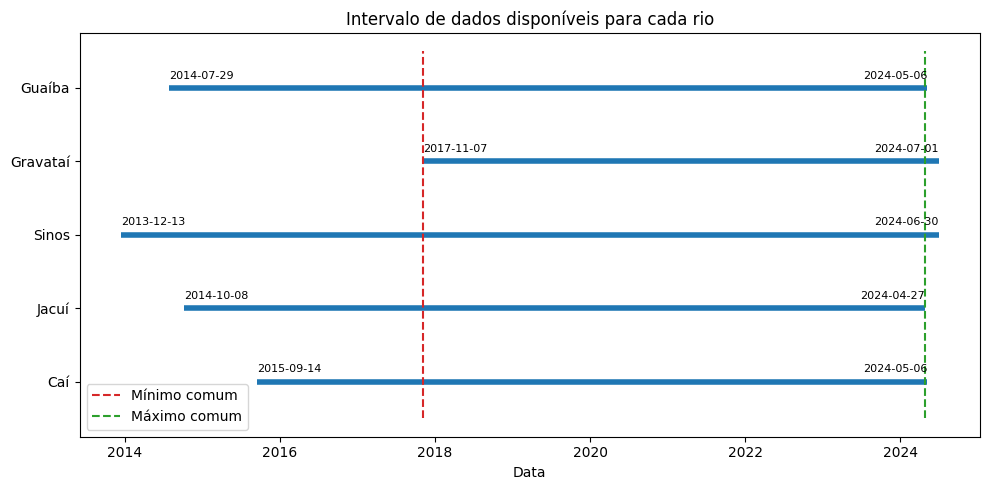
\includegraphics[scale=0.55]{figuras/nivelamento_superior_inferior_dados_rios.png}
	\end{center}
	\fonte{Autor.}
\end{figure}

Extraindo os dados mostrados na Figura \ref{fig:nivelamento_superior_inferior_nivel_rios}, a Tabela \ref{tab:periodo_amostragem} apresenta o período de amostragem de cada uma das fontes de dados dos rios.
\begin{table}[H]
	\centering
	\begin{tabular}{|l|c|c|c|c|}
	\hline
	\textbf{Rio} & \textbf{Data Mínima} & \textbf{Hora Mínima} & \textbf{Data Máxima} & \textbf{Hora Máxima} \\
	\hline
	Rio dos Sinos & 2013-12-13 & 05:00:00 & 2024-06-30 & 09:00:00 \\
	Rio Caí       & 2015-09-14 & 13:00:00 & 2024-05-06 & 14:00:00 \\
	Rio Gravataí  & 2017-11-07 & 12:00:00 & 2024-07-01 & 00:00:00 \\
	Rio Jacuí     & 2014-10-08 & 20:00:00 & 2024-04-27 & 01:00:00 \\
	Lago Guaíba    & 2014-07-29 & 14:00:00 & 2024-05-06 & 14:00:00 \\
	\hline
	\end{tabular}
	\caption{Datas mínima e máxima disponíveis para cada rio analisado}
	\label{tab:periodo_amostragem}
\end{table}

Quanto a base de dados meteorológicos, o site do INMET disponibiliza dados desde o início dos anos 2000 e mantém a base atualizada até os dias atuais, não sendo, portanto, um limitador para a definição do período do dataframe final. Assim, o período de amostragem final pode ser definido a partir de 07 de novembro de 2017, que é a data mínima do rio Gravataí, até 06 de maio de 2024, que é a data máxima do rio Caí, com um dataframe de 56366 linhas.

\section{Transformação dos dados}

A transformação dos dados é uma etapa fundamental para garantir que as informações estejam no formato correto para o treinamento do modelo de previsão. Nesta fase, os dados são convertidos em um formato numérico, adequado para algoritmos de aprendizado de máquina, e normalizados para assegurar que todas as variáveis tenham a mesma escala.

Com os dados meteorológicos e de monitoramento dos rios alinhados, a normalização dos dados é aplicada visando principalmente equilibrar os dados dos níveis dos rios com os dados meteorológicos, tendo em vista que as escalas entre essas informações apresentam uma discrepância maior, pela diferença de unidade de medida entre elas.

Ademais, outro fator que deve ser considerado é se as colunas do \textit{dataframe} são compostas de dados categóricos (geralmente representados através de textos) ou numéricos. Por se tratar de medições aferidas por sensores meteorológicos e/ou geográficos, todas as colunas da base de dados estudada são numéricas.

A partir dessa premissa, a normalização dos dados foi feita utilizando o método \textit{StandardScaler} da biblioteca \textit{Scikit-learn}, que transforma os dados de uma coluna para um valor cuja média seja zero e desvio padrão igual a um. A pontuação padrão de uma amostra x é dada por:

\begin{equation}
z = \frac{x - \mu}{\sigma}
\end{equation}

\noindent onde \( \mu \) é a média da amostra e \( \sigma \) é o desvio padrão. Muitos elementos usados em funções objetivas de \gls{ML} assumem os dados passados para o modelo estão normalizados. No caso do Modelo Ridge, que utiliza um regularizador L2 em sua função objetivo, esse requisito também é necessário, logo, a normalização pelo método \textit{StandardScaler} garante que os recursos estão centrados em torno uma média igual a zero e variação de mesma ordem \cite{scikit_learn_standardscaler}. Caso uma amostra apresente uma variância de magnitude maior do que outros, ele pode dominar a função objetivo e fazer o estimador incapaz de aprender com outros recursos corretamente como esperado.

O método \textit{StandardScaler} também é sensível a \textit{outliers}, que afetam a média e o desvio padrão calculados para a definição dos valores normalizados. Por esse motivo, a aplicação do método \gls{IQR} para remoção dos \textit{outliers}, descrito na seção \ref{sec:limpeza_dos_dados}, além de limpar os dados durante aquela etapa de preparação, garantiu que os dados estivessem mais homogêneos e não fossem distorcidos por valores extremos na normalização desta etapa.

Com os dados normalizados, o \textit{dataframe} está pronto para ser dividido em conjuntos de treinamento e teste, chegando ao estágio final de preparação, e seguindo para o treinamento do modelo de previsão. 

\section{Divisão dos dados em conjuntos de treinamento e teste}

No processo de implementação de um modelo de previsão, a divisão da base de dados em conjuntos de treino e teste constitui a última etapa antes da aplicação do algoritmo, com o objetivo de avaliar a capacidade de generalização do modelo. De maneira geral, a base de dados é dividida em duas partes: uma maior, utilizada para o treinamento do modelo, e uma menor, destinada a testar seu desempenho em dados não observados durante o treinamento. Após a etapa de treinamento com o primeiro conjunto, é possível realizar previsões e compará-las com o segundo conjunto, cujos dados são conhecidos apenas pelo pesquisador. Essa comparação permite a avaliação da performance do modelo por meio do levantamento de métricas de desempenho.

Na divisão dos dados em conjuntos de treinamento e teste, diferentes proporções podem ser utilizadas, dependendo das características do conjunto de dados e do modelo de aprendizado de máquina. Exemplos comuns incluem 80\% dos dados para treinamento e 20\% para teste (80-20), 70\% para treinamento e 30\% para teste (70-30), e 60\% para treinamento e 40\% para teste (60-40) \cite{supri2023asian}.

Não há uma regra geral que defina a melhor divisão entre os conjuntos de treinamento e teste, pois essa escolha pode variar de acordo com o tipo de dado, o modelo utilizado e outros fatores específicos de cada conjunto de informações. No presente trabalho, foi inicialmente adotada a proporção 80:20, com 80\% dos dados para treinamento e 20\% para teste, que produziu bons resultados em trabalhos relacionados \cite{supri2023asian}. Para comparar o desempenho do modelo com outras proporções, também foram testadas as divisões 70:30 e 60:40, a fim de verificar se as métricas de desempenho apresentavam o mesmo comportamento observado no estudo de previsão de preços de ações.

\section{Aplicação do modelo de previsão}

Realizada toda a preparação dos dados, com a divisão em conjuntos de treino e teste e a padronização das variáveis independentes para garantir que todas tenham a mesma escala, o modelo \textit{Ridge} é instanciado no script em Python, com a possibilidade de ajuste de alguns parâmetros para fazer o treinamento e as previsões.

A Regressão \textit{Ridge}, implementada na biblioteca \textit{Scikit-learn} em Python, possui parâmetros ajustáveis que influenciam o desempenho e a robustez do modelo. O principal parâmetro é o alpha, que controla a intensidade da penalização L2, descrita em \ref{sec:regressao-ridge}.

Valores maiores de alpha aumentam a regularização, reduzindo a magnitude dos coeficientes $\hat{\beta}_i$, o que pode levar a \textit{underfitting} ao simplificar excessivamente o modelo. Por outro lado, valores menores aproximam o modelo da regressão linear padrão, com maior risco de \textit{overfitting}. 

O parâmetro \texttt{fit\_intercept} determina se o modelo inclui um termo de intercepto $\beta_0$ na equação de regressão, permitindo que a reta ou hiperplano ajustado não passe necessariamente pela origem (0,0), ou seja, que $y = x$ quando $x = 0$. Quando \texttt{fit\_intercept=True}, o modelo calcula o intercepto para melhor ajustar os dados. 

O parâmetro \texttt{solver} define o método de otimização (como auto, svd, ou cholesky), impactando a eficiência computacional, enquanto \texttt{random\_state} garante reprodutibilidade em solvers que utilizam aleatoriedade. A Figura \ref{fig:exemplo_codigo_ridge} apresenta um trecho de código Python que ilustra a configuração desses parâmetros na implementação da Regressão \textit{Ridge}.

\begin{figure}[H]
	\caption{\label{fig:exemplo_codigo_ridge} Exemplo de código Python para configuração da Regressão Ridge}
	\begin{center}
		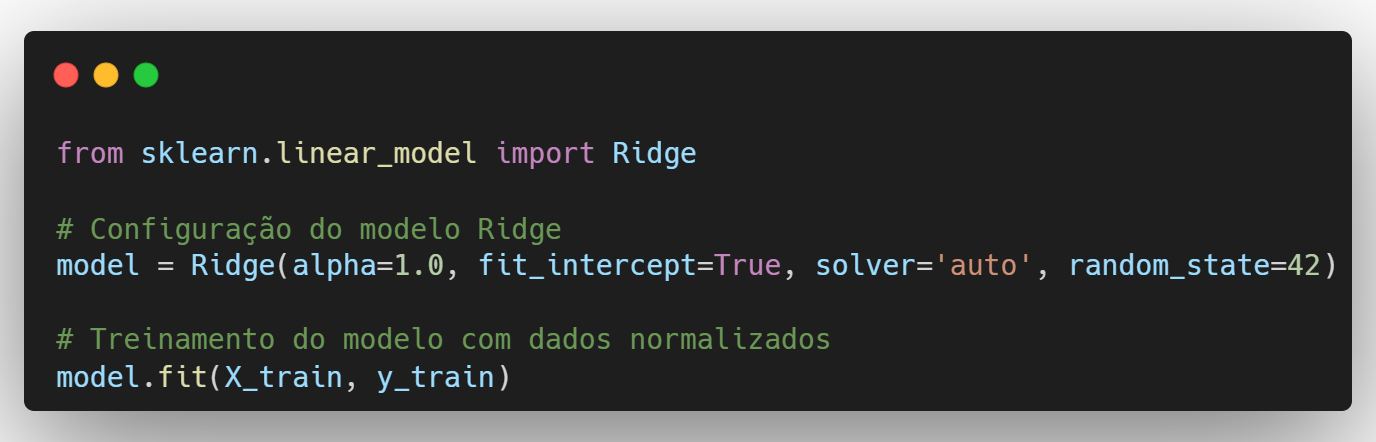
\includegraphics[scale=0.3]{figuras/carbon.png}
	\end{center}
	\fonte{Autor.}
\end{figure}

A implementação prática envolve importar a classe \textit{Ridge}, configurar os hiperparâmetros, treinar o modelo com o método \texttt{fit} e realizar previsões com o método \texttt{predict}. Em \cite{Hastie01102020}, o autor aborda sobre o termo de regularização L2 que penaliza os coeficientes do modelo, explorando o impacto do parâmetro \texttt{alpha} em vários contextos. Em sua tese, é destacado que valores de \texttt{alpha} são geralmente selecionados por validação cruzada, com intervalos típicos variando de 0.01 a 1000, dependendo da escala dos dados e do grau de multicolinearidade. O artigo também menciona que, em aplicações práticas, valores como 0.1, 1 e 10 são frequentemente testados como pontos de partida.

Partindo desse pressuposto, foram testados valores de \texttt{alpha} de 0.001, 0.01, 0.1, 1, 10 e 100, com o objetivo de avaliar o desempenho do modelo em diferentes níveis de regularização. A seguir, são apresentadas as tabelas com os resultados obtidos para cada valor de \texttt{alpha}, considerando as três proporções de divisão dos dados em conjuntos de treinamento e teste: 80:20, 70:30 e 60:40, junto às Figuras X, Y e Z, que ilustram o desempenho do modelo para cada split de treinamento e previsão.

\begin{figure}[H]
	\caption{\label{fig:comparacao_radiacao_nivel_rio}Gráfico modelo de previsão de nível do Lago Guaíba com \texttt{alpha} = 1 e split de treinamento e teste 60:40}
	\begin{center}
		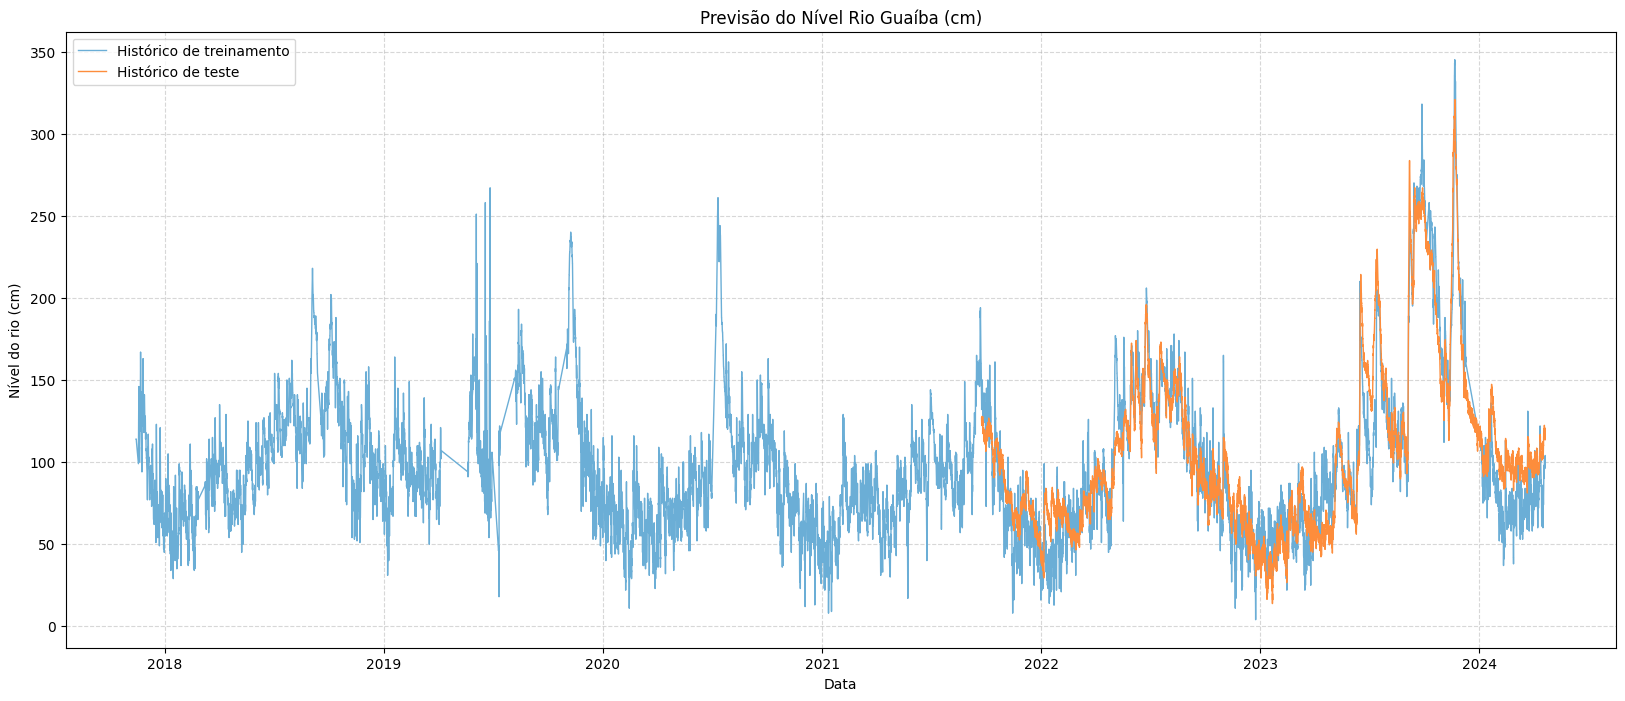
\includegraphics[scale=0.35]{figuras/modelo_previsao_60_40.png}
	\end{center}
	\fonte{Autor.}
\end{figure}

\begin{figure}[H]
	\caption{\label{fig:comparacao_radiacao_nivel_rio}Gráfico modelo de previsão de nível do Lago Guaíba com \texttt{alpha} = 1 e split de treinamento e teste 70:30}
	\begin{center}
		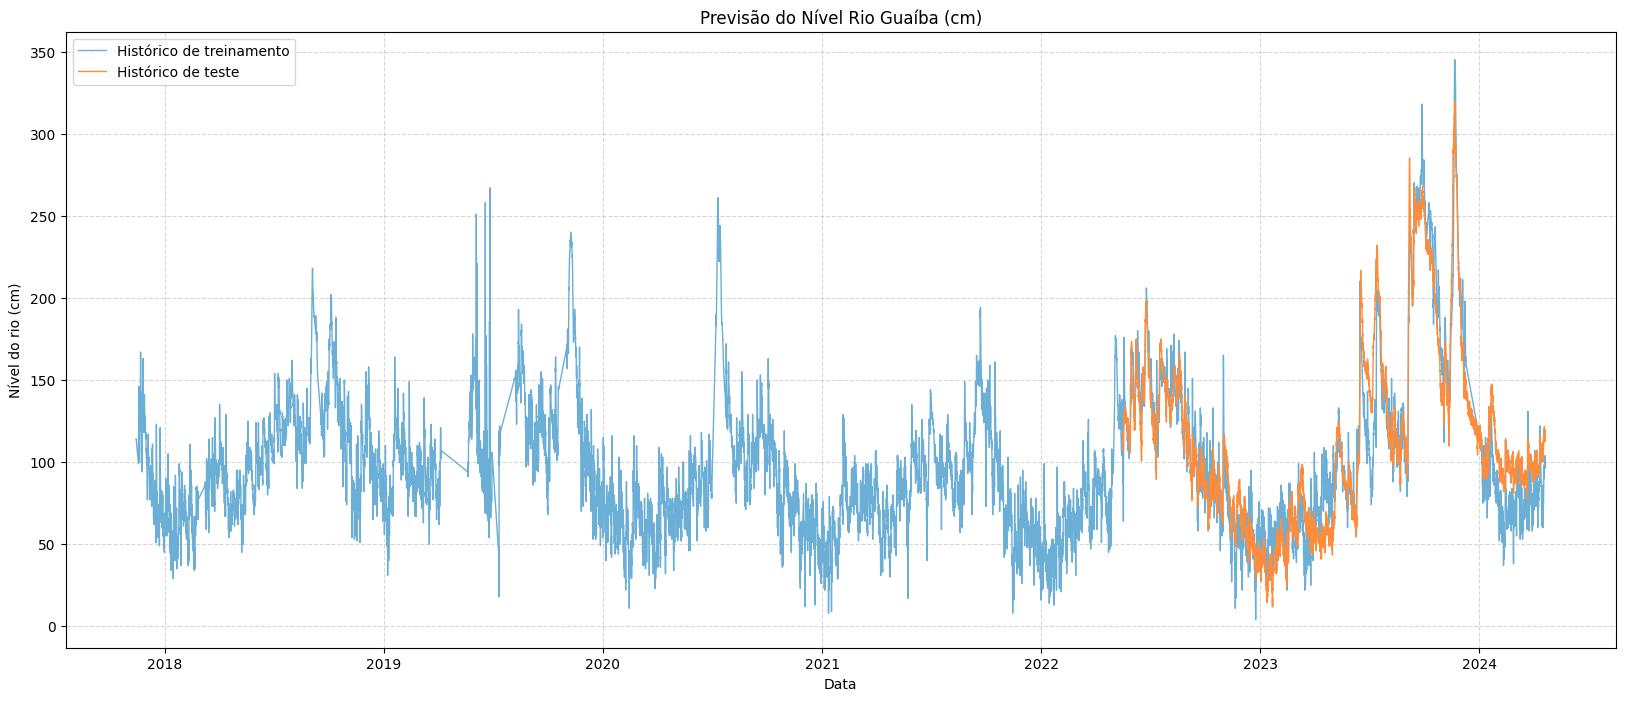
\includegraphics[scale=0.35]{figuras/modelo_previsao_70_30.png}
	\end{center}
	\fonte{Autor.}
\end{figure}

\begin{figure}[H]
	\caption{\label{fig:comparacao_radiacao_nivel_rio}Gráfico modelo de previsão de nível do Lago Guaíba com \texttt{alpha} = 1 e split de treinamento e teste 80:20}
	\begin{center}
		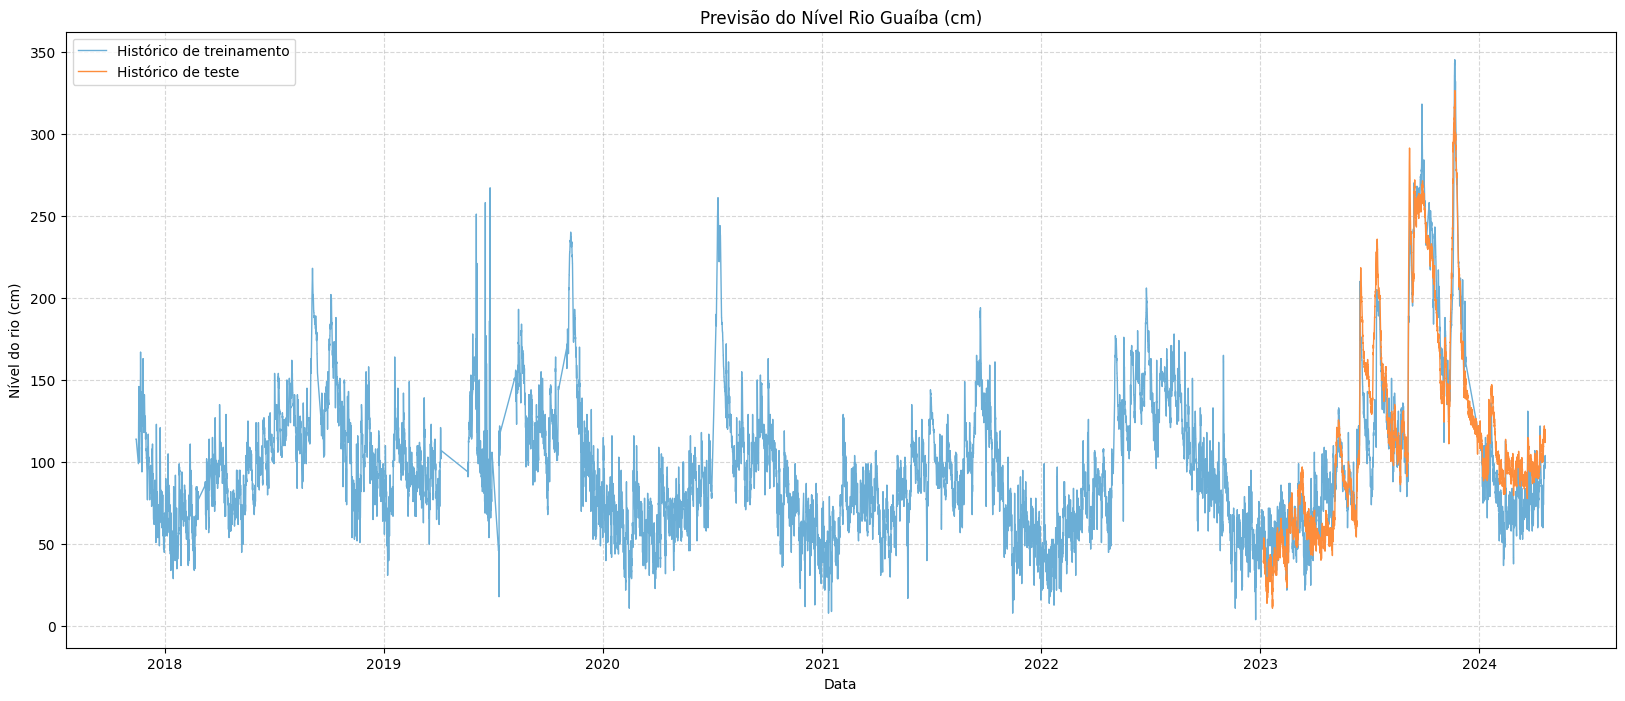
\includegraphics[scale=0.35]{figuras/modelo_previsao_80_20.png}
	\end{center}
	\fonte{Autor.}
\end{figure}

\begin{table}[H]
\centering
\begin{tabular}{|c|c|c|c|c|}
\hline
\textbf{Alpha} & \multicolumn{4}{|c|}{\textbf{0.001}} \\
\hline
\textbf{Split} & \textbf{MSE} & \textbf{RMSE} & \textbf{MAE} & \textbf{R2} \\
\hline
\textbf{80:20} & 456.72 & 21.27 & 16.81 & 0.89 \\
\textbf{70:30} & 372.44 & 19.30 & 15.00 & 0.88 \\
\textbf{60:40} & 379.64 & 19.48 & 15.14 & 0.87 \\
\hline
\end{tabular}
\caption{Tabela de avaliação de desempenho do modelo com alpha 0.01}
\end{table}

\begin{table}[H]
\centering
\begin{tabular}{|c|c|c|c|c|}
\hline
\textbf{Alpha} & \multicolumn{4}{|c|}{\textbf{0.001}} \\
\hline
\textbf{Split} & \textbf{MSE} & \textbf{RMSE} & \textbf{MAE} & \textbf{R2} \\
\hline
\textbf{80:20} & 456.72 & 21.27 & 16.81 & 0.89 \\
\textbf{70:30} & 372.44 & 19.30 & 15.00 & 0.88 \\
\textbf{60:40} & 379.64 & 19.48 & 15.14 & 0.87 \\
\hline
\end{tabular}
\caption{Tabela de avaliação de desempenho do modelo com alpha 0.1}
\end{table}

\begin{table}[H]
\centering
\begin{tabular}{|c|c|c|c|c|}
\hline
\textbf{Alpha} & \multicolumn{4}{|c|}{\textbf{0.001}} \\
\hline
\textbf{Split} & \textbf{MSE} & \textbf{RMSE} & \textbf{MAE} & \textbf{R2} \\
\hline
\textbf{80:20} & 456.72 & 21.27 & 16.81 & 0.89 \\
\textbf{70:30} & 372.44 & 19.30 & 15.00 & 0.88 \\
\textbf{60:40} & 379.65 & 19.48 & 15.14 & 0.87 \\
\hline
\end{tabular}
\caption{Tabela de avaliação de desempenho do modelo com alpha 1}
\end{table}

\begin{table}[H]
\centering
\begin{tabular}{|c|c|c|c|c|}
\hline
\textbf{Alpha} & \multicolumn{4}{|c|}{\textbf{0.001}} \\
\hline
\textbf{Split} & \textbf{MSE} & \textbf{RMSE} & \textbf{MAE} & \textbf{R2} \\
\hline
\textbf{80:20} & 456.72 & 21.27 & 16.81 & 0.89 \\
\textbf{70:30} & 372.44 & 19.30 & 15.00 & 0.88 \\
\textbf{60:40} & 379.64 & 19.48 & 15.14 & 0.87 \\
\hline
\end{tabular}
\caption{Tabela de avaliação de desempenho do modelo com alpha 10}
\end{table}

\begin{table}[H]
\centering
\begin{tabular}{|c|c|c|c|c|}
\hline
\textbf{Alpha} & \multicolumn{4}{|c|}{\textbf{0.001}} \\
\hline
\textbf{Split} & \textbf{MSE} & \textbf{RMSE} & \textbf{MAE} & \textbf{R2} \\
\hline
\textbf{80:20} & 456.73 & 21.27 & 16.81 & 0.89 \\
\textbf{70:30} & 372.45 & 19.30 & 15.00 & 0.88 \\
\textbf{60:40} & 379.65 & 19.48 & 15.14 & 0.87 \\
\hline
\end{tabular}
\caption{Tabela de avaliação de desempenho do modelo com alpha 100}
\end{table}


\chapter{Análise dos resultados}

Uma das formas de avaliar o desempenho de um modelo de aprendizado de máquina é através da análise das métricas de desempenho, que indicam a capacidade do modelo de generalizar e prever corretamente os dados. As métricas de avaliação utilizadas neste trabalho incluem o erro quadrático médio (MSE), a raiz do erro quadrático médio (RMSE), o erro absoluto médio (MAE) e o coeficiente de determinação (R²), onde cada uma delas possui uma interpretação específica:

\begin{itemize}
	\item Erro Quadrático Médio (MSE): Mede a média dos quadrados dos erros, penalizando erros maiores. É útil para entender a magnitude do erro, porém não é intuitiva em termos da escala dos dados, neste caso medido em centímetros.
	\item Raiz do Erro Quadrático Médio (RMSE): É a raiz quadrada do MSE, expressa na mesma unidade dos dados, facilitando a interpretação.
	\item Erro Absoluto Médio (MAE): Mede a média dos erros absolutos, sendo menos sensível a outliers do que o MSE.
	\item R² (Coeficiente de Determinação): Indica a proporção da variância dos dados explicada pelo modelo. Varia de 0 a 1, onde 1 significa ajuste perfeito.
\end{itemize}

Com isso, as tabelas apresentadas mostram que o MSE e o RMSE diminuem conforme o \textit{split} de treinamento diminui e o \textit{split} de teste aumenta. Tal comportamento indica que, à medida que mais dados são utilizados para treinamento, o modelo passa a ter um sobreajuste (\textit{overfitting}), perdendo a capacidade de generalizar e, em vez disso, se adequando estritamente ao conjunto de dados de treinamento.

Quanto ao R², o valor obtido possui uma baixa variação entre os ensaios com diferentes valores de \texttt{alpha} e \textit{split}, ficando entre 0.87 e 0.89. Isso indica que 87\% a 89\% da variância dos dados da variável dependente é explicada pelo modelo. Em outras palavras, o modelo captura a maior parte dos padrões nos dados, deixando apenas 11\% a 13\% da variância como não explicada (devido a ruído, variáveis omitidas ou outros fatores). Um coeficiente de determinação próximo a 1 sugere que o modelo é robusto e confiável para o conjunto de dados analisado. Boa parte dessa robustez se dá pelo tratamento e limpeza dos dados, somada à a correlação entre as variáveis preditoras e a variável dependente.

Em relação ao parâmetro \texttt{alpha}, os resultados mostram que o modelo apresenta um desempenho semelhante para os valores de 0.001, 0.01, 0.1 e 1, com pequenas variações nas métricas de desempenho. Existem alguns fatores que levam a esse comportamento, como a baixa sensibilidade à regularização nos dados, intervalo de \texttt{alpha} insuficiente para notar diferenças significativas ou baixa multicolinearidade entre as variáveis preditoras. Alguns outros fatores como escala dos dados ou tamanho e qualidade do conjunto foram descartados, uma vez que ao longo do trabalho, evidenciam-se os procedimentos realizados para evitar este tipo de falha no modelo.

Uma forma de testar se o modelo possui uma sensibilidade maior à regularização seria aumentar o intervalo de valores de \texttt{alpha} e/ou expor o modelo a mais dados de teste. Tomando um valor muito maior de \texttt{alpha} em relação ao intervalo utilizado anteriormente, foram obtidos os seguintes resultados:

\begin{table}[H]
\centering
\begin{tabular}{|c|c|c|c|c|}
\hline
\textbf{Alpha} & \multicolumn{4}{|c|}{\textbf{1000000}} \\
\hline
\textbf{Split} & \textbf{MSE} & \textbf{RMSE} & \textbf{MAE} & \textbf{R2} \\
\hline
\textbf{80:20} & 469.82 & 21.68 & 16.93 & 0.88 \\
\textbf{70:30} & 379.54 & 19.48 & 15.00 & 0.88 \\
\textbf{60:40} & 391.98 & 19.80 & 15.31 & 0.87 \\
\hline
\end{tabular}
\caption{Tabela de avaliação de desempenho do modelo com alpha 1000000.}
\end{table}

A partir das métricas de avaliação apresentadas, nota-se novamente que o aumento do valor de \texttt{alpha} resultou em um desempenho similar ao observado anteriormente, com erros um pouco maiores, e coeficientes de determinação próximos. Assim, em casos onde uma grande variação de \texttt{alpha} permanece com resultados semelhantes, tal comportamento indica que o modelo já atingiu seu ponto de saturação, obtendo um desempenho ótimo para baixos termos de regularização.

Considerando que a base de dados utilizada possui uma frequência temporal em horas, o modelo realiza uma previsão do nível do Lago Guaíba para o próximo período de uma hora, com base nos dados meteorológicos e do monitoramento dos rios daquela amostra temporal. Pensando em uma previsão com frequência diária, o modelo foi ajustado para ter um intervalo de previsão de 24 horas. Assim, ao prever o nível do lago na hora "00:00", a próxima previsão desconsidera as os registros das 23 horas seguintes, realizando uma nova previsão no dia seguinte, com dados meteorológicos e dos demais rios também somente do outro dia. Na Tabela \ref{tab:monthly_summary}, é mostrado um resumo mensal das previsões do modelo, agregandos as previsões diárias de cada mês como uma média e comparando os valores reais e previstos do nível do lago, além da diferença absoluta e percentual entre eles.

\begin{table}[H]
\centering
\begin{tabular}{|c|c|c|c|c|}
	\hline
	\textbf{Mês/Ano} &  \textbf{Atual(cm)} &  \textbf{Previsto(cm)} &  \textbf{Diferença(cm)} &  \textbf{Diferença(\%)} \\
	\hline
	05/2022 & 126.62 & 125.83 & \textcolor{BrickRed}{-0.79} & \textcolor{BrickRed}{-0.62} \\
06/2022 & 157.60 & 150.06 & \textcolor{BrickRed}{-7.54} & \textcolor{BrickRed}{-4.78} \\
07/2022 & 139.67 & 140.09 & \textcolor{ForestGreen}{+0.42} & \textcolor{ForestGreen}{+0.30} \\
08/2022 & 137.95 & 139.59 & \textcolor{ForestGreen}{+1.64} & \textcolor{ForestGreen}{+1.19} \\
09/2022 & 102.62 & 99.25 & \textcolor{BrickRed}{-3.37} & \textcolor{BrickRed}{-3.28} \\
10/2022 & 85.76 & 81.89 & \textcolor{BrickRed}{-3.87} & \textcolor{BrickRed}{-4.51} \\
11/2022 & 64.00 & 79.35 & \textcolor{ForestGreen}{+15.35} & \textcolor{ForestGreen}{+23.98} \\
12/2022 & 53.69 & 51.27 & \textcolor{BrickRed}{-2.42} & \textcolor{BrickRed}{-4.51} \\
01/2023 & 51.08 & 36.35 & \textcolor{BrickRed}{-14.73} & \textcolor{BrickRed}{-28.84} \\
02/2023 & 62.91 & 55.49 & \textcolor{BrickRed}{-7.42} & \textcolor{BrickRed}{-11.79} \\
03/2023 & 58.01 & 67.77 & \textcolor{ForestGreen}{+9.76} & \textcolor{ForestGreen}{+16.82} \\
04/2023 & 78.50 & 56.32 & \textcolor{BrickRed}{-22.18} & \textcolor{BrickRed}{-28.25} \\
05/2023 & 94.21 & 93.28 & \textcolor{BrickRed}{-0.93} & \textcolor{BrickRed}{-0.99} \\
06/2023 & 113.47 & 124.27 & \textcolor{ForestGreen}{+10.80} & \textcolor{ForestGreen}{+9.52} \\
07/2023 & 138.53 & 162.85 & \textcolor{ForestGreen}{+24.32} & \textcolor{ForestGreen}{+17.56} \\
08/2023 & 115.04 & 111.91 & \textcolor{BrickRed}{-3.13} & \textcolor{BrickRed}{-2.72} \\
09/2023 & 229.53 & 218.44 & \textcolor{BrickRed}{-11.09} & \textcolor{BrickRed}{-4.83} \\
10/2023 & 220.16 & 200.87 & \textcolor{BrickRed}{-19.29} & \textcolor{BrickRed}{-8.76} \\
11/2023 & 201.79 & 202.08 & \textcolor{ForestGreen}{+0.29} & \textcolor{ForestGreen}{+0.14} \\
12/2023 & 149.75 & 134.52 & \textcolor{BrickRed}{-15.23} & \textcolor{BrickRed}{-10.17} \\
01/2024 & 95.98 & 110.42 & \textcolor{ForestGreen}{+14.44} & \textcolor{ForestGreen}{+15.04} \\
02/2024 & 67.41 & 91.07 & \textcolor{ForestGreen}{+23.66} & \textcolor{ForestGreen}{+35.10} \\
03/2024 & 76.78 & 90.61 & \textcolor{ForestGreen}{+13.83} & \textcolor{ForestGreen}{+18.01} \\
04/2024 & 86.68 & 98.16 & \textcolor{ForestGreen}{+11.48} & \textcolor{ForestGreen}{+13.24} \\
\hline
\end{tabular}
\caption{Diferença entre os valores reais e previstos do nível do Lago Guaíba}
\label{tab:monthly_summary}
\end{table}

\begin{figure}[H]
	\caption{\label{fig:diferencas_previsao_lago_guaiba}Diferenças entre os valores reais e previstos do nível do Lago Guaíba}
	\begin{center}
		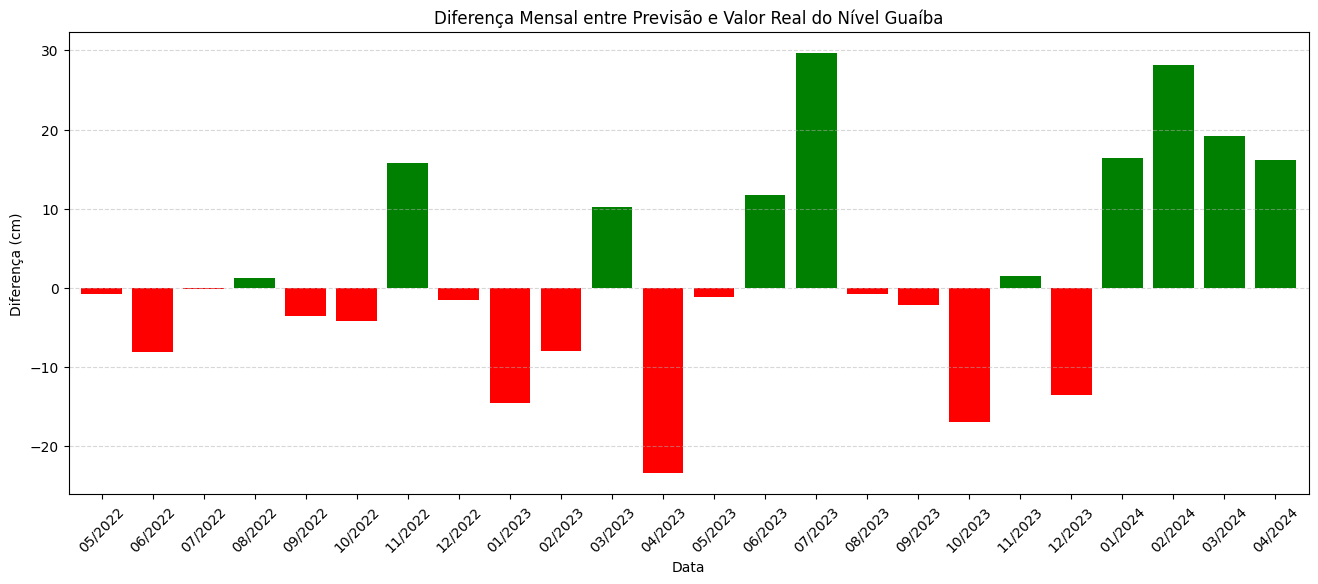
\includegraphics[scale=0.45]{figuras/diferencas_previsao_lago_guaiba.png}
	\end{center}
	\fonte{Autor.}
\end{figure}

Com base na Tabela \ref{tab:monthly_summary} e na Figura \ref{fig:diferencas_previsao_lago_guaiba}, é possível observar que, embora os erros não se acumulem a cada mês, eles se tornam maiores de forma geral, conforme a previsão se afasta do início do teste. A o maior erro ocorreu em julho de 2024, com uma diferença de 24.32 cm em relação ao valor real do nível do lago, o que representa uma diferença percentual de 17.56\%. Por outro lado, o menor erro ocorreu em julho de 2022, com uma diferença de apenas 0.42 cm, ou 0.30\% em relação ao valor real.

Outro ponto a ser destacado é que, 14 dos 24 meses analisados, o modelo apresentou uma previsão com erro negativo, ou seja, o valor previsto foi menor que o valor real do nível do lago. Isso pode indicar que o modelo tende a subestimar os níveis do lago, sendo um fator de risco no alerta para enchentes e inundações, uma vez que a previsão de níveis mais baixos pode levar a uma resposta inadequada em situações de emergência. Por outro lado, mesmo com a subestimação, 8 dos 14 meses com erro negativo apresentaram uma diferença percentual inferior a 5\%, o que pode ser considerado aceitável em termos de previsão. 

Utilizando outras pesquisas de previsão do nível de rios para fins comparativos, um estudo que implementou um modelo de Rede Neural do tipo Long Short-Term Memory (LSTM), para a previsão do rio Tisza, na Hungria. De forma geral, o modelo obteve um erro absoluto médio que variou de 4,2 cm no 1º dia de previsão, até 34,7 cm no 7º dia. Outra análise feita no estudo mostrou que entre 68,5\% e 76,1\% das previsões ficaram dentro dos intervalos de precisão exigidos para os diferentes dias da previsão de 7 dias à frente. Estes intervalos eram progressivos, sendo o primeiro dia com tolerância de 5cm, a partir do 3º dia com tolerância de 15cm, no 5º dia com tolerância de 25cm e por fim no 7º dia com tolerância de 35cm \cite{Vizi2023}.

Comparando com este Artigo, o modelo \textit{Ridge}, embora tenha oscilado nas previsões, gerando um grau de incerteza no desempenho,apresentou resultados gerais melhores em termos de erro absoluto médio, especialmente nos dias mais distantes de previsão.